%%%%%%%%%%%%%%%%%%%%%%%%%%%%%%%%%%%%%%%%%%%%%%%%%%%%%%%%%%%%%%%%%%%%%%%%%%%%
%% Author style for Mathematics of Operations Research (moor)
%% Mirko Janc, Ph.D., INFORMS, pubtech@informs.org
%% ver. 0.9, March 2005
%%%%%%%%%%%%%%%%%%%%%%%%%%%%%%%%%%%%%%%%%%%%%%%%%%%%%%%%%%%%%%%%%%%%%%%%%%%%
\documentclass{article}              % for a regular run
%\documentclass[moor,nonblindrev]{informs1} % for review, not blinded
%\documentclass[moor,blindrev]{informs1}    % for review, blinded
%\documentclass[moor,copyedit]{informs1}    % spaced for copyediting
\usepackage{graphicx}
% If hyperref is used, dvi-to-ps driver of choice must be declared as
%   an additional option to the \documentstyle. For example
%\documentclass[dvips,moor]{informs1}      % if dvips is used 
%\documentclass[dvipsone,moor]{informs1}   % if dvipsone is used, etc. 

% Private macros here (check that there is no clash with the style)
\usepackage{amsmath}
\usepackage{amsthm}
\usepackage{amsfonts}
\usepackage{amssymb}
\usepackage{algorithm2e}
% Natbib setup for numeric style
\usepackage{natbib}
 \def\bibfont{\small}%
 \def\bibsep{\smallskipamount}%
 \def\bibhang{24pt}%
 \def\BIBand{and}%
 \def\newblock{\ }%
 \bibpunct[, ]{[}{]}{,}{n}{}{,}%

%% Hyperref setup
\usepackage[colorlinks=true,breaklinks=true,bookmarks=true,urlcolor=blue,
     citecolor=blue,linkcolor=blue,bookmarksopen=false,draft=false]{hyperref}

\def\EMAIL#1{\href{mailto:#1}{#1}}% When hyperref is used, otherwise outcomment 
\def\URL#1{\href{#1}{#1}}         % When hyperref is used, otherwise outcomment 

%% Setup of theorem styles. Outcomment only one. 
%% Preferred default is the first option.
%\TheoremsNumberedByChapter  % (Theorem 1.1, Lema 1.1, Theorem 1.2)

%% Setup of the equation numbering system. Outcomment only one.
%% Preferred default is the first option.
%\EquationsNumberedBySection % (1.1), (1.2), ...

% In the reviewing and copyediting stage enter the manuscript number.
%\MANUSCRIPTNO{} % When the article is logged in and DOI assigned to it,
                 %   this manuscript number is no longer necessary

\newcommand{\tbd}[1]{{ \bf [ TBD #1 ]}}

\global\long\def\P{\mathbb{P}}%
\global\long\def\N{\mathbb{N}}%
\global\long\def\U{\mathbb{U}}%
\global\long\def\E{\mathbb{E}}%
\global\long\def\R{\mathbb{R}}%
\global\long\def\G{\mathcal{G}}%
\global\long\def\g{\mathbb{\Pi}}%
\global\long\def\F{\mathcal{F}}%
\global\long\def\S{\mathcal{S}}%
\global\long\def\Q{\mathcal{Q}}%
\global\long\def\B{\mathcal{B}}%
\global\long\def\ND{\mathcal{N}}%
\global\long\def\XX{\mathcal{X}}%
\global\long\def\indep#1{{\perp\hspace{-2mm}\perp}#1}%
\global\long\def\L{\mathcal{L}}%
\global\long\def\var{\mathrm{var}}%
\global\long\def\cov{\mathrm{cov}}%
\global\long\def\charf{\mathbf{1}}%
\global\long\def\d{\mathrm{d}}%
\global\long\def\M{\mathcal{M}}%
\global\long\def\T{\mathcal{T}}%
\global\long\def\Exp{\mathrm{Exp}}%
\global\long\def\Uniform{\mathrm{U}}%
\global\long\def\eqd{{d\atop =}}%
\global\long\def\A{\mathcal{A}}%
\global\long\def\I{\mathcal{I}}%
\global\long\def\X{\mathcal{X}}%
\global\long\def\supp{\mathrm{support}}%
\global\long\def\H{\mathcal{H}}%
\global\long\def\Z{\mathcal{Z}}%
\global\long\def\as{\qquad a.s.}%
\global\long\def\on{\qquad\text{on }}%
\global\long\def\C{\mathcal{C}}%
\global\long\def\barxi{\overline{\xi}}%
\global\long\def\Po{\mathrm{Po}}%
\global\long\def\barvs{\overline{\varsigma}}%
\global\long\def\bareps{\overline{\varepsilon}}%
\global\long\def\bari{\overline{\iota}}%
\global\long\def\barx{\overline{x}}%
\global\long\def\baru{\overline{u}}%
\global\long\def\bars{\overline{s}}%
\global\long\def\Bi{\mathrm{Bi}}%
\global\long\def\defined{\stackrel{\text{\rm def}}{=}}%
\global\long\def\dw{\mathrm{d}}%
\global\long\def\bary{\overline{y}}%
\global\long\def\cvar{\mathrm{CVaR}}%
\global\long\def\d{\mathbf{d}}%
%\global\long\def\qed{} %{$\Box$ \bigskip}%

\newtheorem{definition}{Definition}
\newtheorem{lemma}{Lemma}
\newtheorem{example}{Example}
\newtheorem{theorem}{Theorem}
\newtheorem{proposition}{Proposition}
\newtheorem{remark}{Remark}
\newtheorem{corollary}{Corollary}

\newcommand{\refauthor}[1]{\uppercase{#1}}
\newcommand{\reftitle}[1]{\emph{#1}}
\newcommand{\refyear}[1]{#1}
\newcommand{\refvolume}[1]{vol. #1}
\newcommand{\refissue}[1]{iss. #1}
\newcommand{\refjournal}[1]{#1}
\newcommand{\refpages}[1]{pp. #1}
\newcommand{\refisbn}[1]{ISBN #1}
\newcommand{\refpublisher}[1]{#1}
\newcommand{\refurl}[1]{Available at: \url{#1}}
\newcommand{\refcopyright}[1]{\copyright #1}
\newcommand{\refdate}[1]{[cit. #1]}
\newcommand{\refsw}{[software]}

%%%%%%%%%%%%%%%%
\begin{document}
%%%%%%%%%%%%%%%%

% Outcomment only when entries are known. Otherwise leave as is and 
%   default values will be used.
%\setcounter{page}{1}
%\VOLUME{00}%
%\NO{0}%
%\MONTH{Xxxxx}% (month or a similar seasonal id)
%\YEAR{0000}% e.g., 2005
%\FIRSTPAGE{000}%
%\LASTPAGE{000}%
%\SHORTYEAR{00}% shortened year (two-digit)
%\ISSUE{0000} %
%\LONGFIRSTPAGE{0001} %
%\DOI{10.1287/xxxx.0000.0000}%

% Author's names for the running heads
% Sample depending on the number of authors;
% \RUNAUTHOR{Jones}
% \RUNAUTHOR{Jones and Wilson}
% \RUNAUTHOR{Jones, Miller, and Wilson}
% \RUNAUTHOR{Jones et al.} % for four or more authors
% Enter authors following the given pattern:
%\RUNAUTHOR{M. \v Sm\'\i d and V. Kozm\'\i k}

% Title or shortened title suitable for running heads. Sample:
% \RUNTITLE{Bundling Information Goods of Decreasing Value}
% Enter the (shortened) title:
%\RUNTITLE{Approximation of Multistage Stochastic Programming Problems by Smoothed
%Quantization}

% Full title. Sample:
% \TITLE{Bundling Information Goods of Decreasing Value}
% Enter the full title:
\title{Approximation of Multistage Stochastic Programming Problems by Smoothed Quantization}

% Block of authors and their affiliations starts here:
% NOTE: Authors with same affiliation, if the order of authors allows, 
%   should be entered in ONE field, separated by a comma. 
%   \EMAIL field can be repeated if more than one author
%\author{Martin \v Sm\'\i d\footnote{Czech Academy of Sciences, Institute of Information Theory and Automation, Pod Vodárenskou věží 4, 18200 Praha 8, Czech Republic, corresponding author, smid@utia.cas.cz}, V\'aclav Kozm\'\i k\footnote{Czech Academy of Sciences, Institute of Information Theory and Automation, Pod Vodárenskou věží 4, 18200 Praha 8, Czech Republic }}

% Enter all authors
 % end of the block


%

% Sample
%\KEYWORDS{deterministic inventory theory; infinite linear programming duality; 
%  existence of optimal policies; semi-Markov decision process; cyclic schedule}
%\MSCCLASS{Primary: 90B05; secondary: 90C40, 90C90}
%\ORMSCLASS{Primary: Inventory/production: deterministic multi-item;
%  secondary: dynamic programming/optimal control: deterministic 
%  semi-Markov; programming: infinite dimensional}
%\HISTORY{Received November 20, 2003; revised March 8, 2004, and March 26, 2004.}

% Fill in data. If unknown, outcomment the field
%\ORMSCLASS{stochastic programming; dynamic programming models}
%\HISTORY{}

\maketitle
%\end{document}
\begin{abstract}
We present an approximation technique for solving multistage stochastic programming problems with Markov underlying stochastic process. The process is approximated by a discrete skeleton process, which is consequently smoothed down by means of the original unconditional distribution. Approximated this way, the problem is solvable by Markov Stochastic Dual Dynamic Programming. We state an upper bound of the nested distance of the exact process and its approximation and discuss its convergence in the one-dimensional case. Further, we propose an adjustment of the approximation guaranteeing boundedness of the approximate problem. Finally, we apply our technique to a real-life  production-emission trading problem and demonstrate the performance of its approximation given the ``true'' distribution of the random parameters.
\end{abstract}

\noindent Key words: multistage stochastic programming; approximation; Markov dependence; SDDP

\noindent AMS class: 90C15

\section{Introduction.}

Stochastic programming evolved from its deterministic counterpart by realizing that the parameters influencing the objective function and constraints are usually uncertain, coming from the real world around us. Real world applications are ranging from economy to biology or logistics and engineering. The development in field led to multi-stage stochastic programming, which allows multiple stages of the decision and data process. Such models capture the dynamics of the underlying random process, and we are allowed to adjust our decisions based on the random parameters observed so far. Our decisions cannot depend on the parameters which are still uncertain and will be resolved in future stages, which means that the decisions fulfill the notion of nonanticipativity. Even though this generalization can be described in a straightforward manner, it brings substantial issues with theoretical properties, random process models and tractability. The applicability of such models often depends on the structure of the problem we are trying to solve. Multi-stage stochastic models have provided valuable improvements over the two-stage models in some particular cases, usually involving some complex time-dependent structure. Such examples can be found, for instance, in finance, energy management or transportation.

There are two common ways to describe uncertainty in the stochastic programming models. The first approach is to collect some historical values or experts' opinion and produce a discrete distribution, which consists of scenarios with assigned probabilities. The second approach is to assume that the random inputs follow some continuous distribution and estimate its parameters from the data or use the experts' opinion to choose the parameters. When a continuous distribution is selected, sampling methods are commonly used to convert it to the discrete version in order to obtain a numerically tractable approximation, see for example \cite{pflug2014multistage}. For large-scale problems, we are unable to compute precise solutions even for this discrete approximation. 

Most of the stochastic programming models optimize the expected outcome of the random costs or returns. Resulting decisions are optimal on average, but possible risks are neglected. In many cases, this does not have to be an appropriate goal, as these decisions could produce a very unsatisfactory performance or even lead to bankruptcy under the worst-case scenarios. First developments in modeling risk aversion by using utility functions can be found in Bernoulli \cite{bernoulli}, or, more formal and precise description, in von Neumann and Morgenstern \cite{neumann}. Other significant ways to producing more robust solutions include mean-risk models. These bi-criteria models aim to find an efficient solution with respect to maximization of the mean return and minimization of the risk which is linked to the future uncertainty. Basics of the mean-risk concept using  variance and semivariance as a measure of risk were published in the article \cite{markowitz_artic} and  book \cite{markowitz_book}  by Harry Markowitz already in the 1950s. In recent years, risk-averse stochastic optimization based on various risk measures has received significant attention. The properties required of {\em coherent} risk measures, introduced in Artzner et al.\ \cite{artzner_99}, are now widely accepted for time-static risk-averse optimization. One of the most popular risk measures, Conditional Value at Risk (CVaR, see Rockafellar and Uryasev \cite{rockafellar2002conditional}), is known to satisfy these properties; for an overview of many others see, for instance, Krokhmal et al.\ \cite{K-U-Z}. A number of proposals have been put forward to extend the concept of coherent risk measures to handle multi-stage stochastic optimization.

Due to the complexity of stochastic programs,  discussed for example in Shapiro and Nemirovski \cite{complexity}, approximations are often employed. Monte Carlo sampling and scenario approximations have been used even before they got a name of \emph{Sample Average Approximation} in the article of Kleywegt et al. \cite{saa}. Approximate solutions depend on the particular set of sampled scenarios and are therefore random in general. Such approximate solutions require statistical validation, which is usually based on doing multiple replications and examining the stability of solutions and objective values, see Bayraksan and Morton \cite{bayraksan_morton_2011} for a summary of available methods. Scenario-based stochastic programs can often be reformulated as one large-scale standard optimization program, and such program can be solved directly by solvers like CPLEX, Gurobi or COIN-OR. The reformulated programs are usually very large and require long solving times or are unsolvable at all. This motivated the development of algorithms which exploit the special structure of stochastic programs and take advantage of particular properties like convexity. Optimization problems which include integer variables are known to be very hard to solve in general, and they are, of course, even more demanding in the stochastic setting. Most of the recent algorithms employ a technique of building so-called cuts on the feasible space or objective function. These cuts are used to eliminate infeasible or suboptimal decisions, or to approximate the objective function. The basic algorithm -- Benders' decomposition, sometimes called L-shaped method, was developed by Benders \cite{benders}, see also Van Slyke and Wets \cite{slyke_wets}. There have been many improvements of the basic algorithm, especially the multicut method by Birge and Louveaux \cite{birge_multicut}, regularized decomposition by Ruszczy{\'n}ski \cite{regular_decomp} and stochastic decomposition by Higle et al. \cite{stochdecomp_2stage}. These decomposition algorithms usually provide approximate solution and control its quality by computing lower and upper bounds on the true optimal objective value.

The structure of recourse functions in the multi-stage stochastic programs is particularly difficult from the algorithmic perspective. If we transform the multi-stage stochastic program into the dynamic programming recursion, the last stage program can be solved by the algorithms mentioned above. For the preceding stages, we need to realize that the precise form of the recourse function cannot be obtained, and we need to rely only on its approximation, provided by the cuts. Therefore we are recursively accumulating approximation error, which leads to slower convergence and requires further validation of correctness. The basic multi-stage decomposition algorithm, Nested Benders' decomposition  \cite{birge_85}, applied to a multi-stage stochastic program requires computational effort that grows exponentially  in the number of stages. Other important algorithms designed to solve multi-stage stochastic programs include extensions of stochastic decomposition to the multi-stage case \cite{stochdecomp,sen_zhou_2012}, progressive hedging \cite{rockafellar_wets_91} and stochastic dual dynamic programming (SDDP) \cite{pereirapinto}. SDDP will be used as the main solution technique for multi-stage stochastic programs in this article.

SDDP originated in the work of Pereira and Pinto \cite{pereirapinto}, and inspired a number of related algorithms \cite{chen_powell_99,donohue_birge_06,linowsky_philpott_05,philpott_guan_08}, which aim to improve its efficiency. SDDP-style algorithms have computational effort per iteration that grows linearly in the number of stages. To achieve this, SDDP algorithms rely on the assumption of stage-wise independence which is rarely
the case in practice, especially in financial applications. Sometimes
the requirement of time-independence can be circumvented by a suitable
reformulation of the decision problem -- see e.g. \cite{kozmik2014evaluating}
working with (independent) returns rather than (time-dependent) prices or \cite{lohndorf2019modeling} using artificial decision variables;
however, in the majority of real-life applications, nothing like that
could be done. A relatively recent modification of the SDDP
\cite{philpott2013solving}, which we call Markov SDDP, permits the
underlying process to be conditioned by a finite Markov chain, which 
allows to approximate a time-dependent underlying process by a hidden
Markov model. However, as the Markov chain has to be sparse for computational
reasons, the original process is approximated only
roughly, which may result in serious errors. When CVaR is used as a risk measure, the discretized version may completely fail to approximate the original problem because the tails of the distribution are approximated at most by several atoms if not only with a single one, which causes CVaR to degenerate into the worst-case risk measure: instead of a risk averse problem, we would solve a minimax one. 


In this paper, we overcome this problem by proposing a novel approximation technique which we call \emph{smoothed quantization}, consisting of two steps at each stage $t$. In the first step, the exact
(conditional) $t$-th stage distribution is approximated by its quantization,
i.e. an atomic distribution with the probabilities equal to the exact
(conditional) probabilities of pre-chosen regions surrounding its
atoms (see \cite{lohndorf2019modeling}, \cite{kreitmeier2011optimal} or \cite{Pflug01}). In
the second step, the quantization is smoothed down by means of the
exact unconditional distribution, restricted to the regions. As a
result, the shape of the approximation is resembling the one of the original distribution with the first-stage approximation being equal to the original distributuon. The approximating process remains dependent on the past only through a finite number of possible values, which allows us to use the Markov SDDP to solve optimization problems with time-dependent underlying processes (approximated by our technique).

To measure the accuracy of our approximation, we use nested distance, denoted by 
$\d$, which has been specifically designed for multi-stage stochastic programs (see
\cite{pflug2012distance} or \cite{pflug2014multistage}). Under
certain conditions mentioned in \cite{pflug2014multistage}), Theorem 6.1:
\begin{equation}
|v(\xi)-v(\varsigma)|\leq K\d(\xi,\varsigma)\label{eq:tbd}
\end{equation}
where $\text{\ensuremath{\xi} and \ensuremath{\varsigma} }$are the
exact process and its approximation, $K$ is a constant, and $\ensuremath{v(\bullet)}$
is the corresponding value function. This could help us to keep the approximation error (the l.h.s. of (\ref{eq:tbd})) under control, but the abovementioned ``certain conditions'' are rarely
fulfilled in practice. Even though we might expect for (\ref{eq:tbd}) to hold
locally, we demonstrate in the sequel, 
that the left hand side of (\ref{eq:tbd}) is infinite for some approximations $\varsigma$.
Nevertheless, in our opinion, nested distance is still the most
suitable metric for measurement of random parameters approximation in multi-stage stochastic programming.


As the computation of the nested distance for general $\varsigma$ is intractable and even determining the optimal skeleton (in some particular sense of optimality as described in \cite{lohndorf2019modeling}), leads to non-trivial non-convex optimization problems, we give up on finding the optimal approximation. Instead, we state an upper bound
of the nested distance between the exact process and its smoothed
quantization and we show that this distance converges in the one-dimensional
case. Further, we discuss settings of the approximation's parameters so
that the distance is kept small, and propose a refinement of the
approximation guaranteeing that the approximated problem is bounded. 
Finally, we apply our
approximation technique to a real-life optimal production and emission
trading multi-stage problem and test the performance of the approximate
solution w.r.t. the exact distribution of the underlying process.

The paper is organized as follows. After the introduction of the risk-averse
multi-stage problem (Section \ref{sec:Ihtroductiondef}) and the discussion
of the nested distance (Section \ref{sec:Nested}), we introduce the
smoothed quantization (Section \ref{sec:sq}) and we discuss the choice
of its parameters and its refinement (Section \ref{sec:approx}).
Further, the practical illustration is presented (Section \ref{sec:appl})
and the paper is concluded (Section \ref{sec:conc}). Auxiliary results
are put into the Appendix.

\section{\label{sec:Ihtroductiondef} Risk averse multi-stage problem.}

We consider the risk-averse $T$-stage linear stochastic programming
problem:
\begin{equation}\label{eq:p}
\begin{split}
\inf\rho(c'_{0}x_{0},&\dots,c'_{T}x_{T})\\
&x_{0}\in\R_{+}^{d_{0}},\quad A_{0}x_{0}=b_{0},\\
&x_{t}\in\R_{+}^{d_{t}},\quad x_{t}\in\F_{t},\quad A_{t}
\left[\begin{array}{c}
x_{t-1}\\
x_{t}
\end{array}\right]=b_{t},\quad1\leq t\leq T.
\end{split}
\end{equation}
Here, $b_{0}\in\R^{j_{0}},c_{0}\in\R^{d_{0}}$ are deterministic vectors,
$A_{0}\in\R^{j_{0}\times d_{0}}$ is a deterministic matrix. Further,
for each $0<t\leq T$, $b_{t}\in\R^{j_{t}}$ and $c_{t}\in\R^{d_{t}}$ are
(possibly) random vectors and $A_{t}\in\R^{j_{t}\times (d_{t-1} + d_t)}$ is
a (possibly) random matrix. Symbol $'$ denotes transposition. The dimensions, $d_{0},\dots,d_{T}$ and
$j_{0},\dots,j_{T}$ are deterministic. Finally, $(\F_{t})_{t=0,\dots,T}$
is the filtration generated by process $(A_{t},b_{t},c_{t})_{0\leq t\leq T}$,
and $\rho$ is a nested risk measure defined as
\[
\rho(z_{0},\dots,z_{T})=z_{0}+\sigma_{1}(z_{1}+\sigma_{2}(z_{2}\dots+\sigma_{T}(z_{T}))),\qquad z_{t}\in\F_{t},\quad0\leq t\leq T,
\]
where, for each $1\leq t\leq T$, $\sigma_{t}$ is a conditional risk
mapping, i.e. a convex, monotone and translation invariant function
from the space of integrable $\F_{t}$-measurable real functions into
the space of integrable $\F_{t-1}$-measurable real functions (see
\cite{ruszczynski2006conditional}, Definition 2.1). 

One of the most frequent choices of $\sigma_{\bullet}$ is the
mean-CVaR risk mapping, defined as 
\[
\sigma_{t}(z)=(1-\lambda)\E(z|\F_{t-1})+\lambda \cvar_{\alpha}(z|\F_{t-1}),\qquad1\leq t\leq T,
\]
where $0\leq\lambda\leq1$ is a risk-aversion parameter and $\alpha \in [0,1)$
is the CVaR level (see e.g. \cite{rockafellar2002conditional} for
the discussion of CVaR and its evaluation within stochastic programs).

Without loss of generality,\footnote{Recall that non-Markov processes may be transformed to Markov processes by adding their history into the state space.} we assume that
\begin{equation}
A_{t}=\Xi_{t}(\xi_{t},\eta_{t}),\qquad b_{t}=\phi_{t}(\xi_{t},\eta_{t}),\qquad c_{t}=\psi_{t}(\xi_{t},\eta_{t}),\qquad0\leq t\leq T,\label{eq:exi}
\end{equation}
where $\xi$ is a Markov process taking values in $\R^{p}$ with
$\xi_{0}$ deterministic, $\eta$ is a time-independent stochastic
process taking values in $\R^{q}$ with $\eta_{0}$ deterministic,
independent of $\xi$, and, for each $0\leq t\leq T$, $\Xi_{t}:\R^{p+q}\rightarrow\R^{j_{t}\times (d_{t-1}+d_{t}) },$
 $\phi_{t}:\R^{p+q}\rightarrow\R^{j_{t}}$ and $\psi_{t}:\R^{p+q}\rightarrow\R^{d_{t}}$
are measurable mappings.

As it was already mentioned, the computationally easiest situation is when the random parameter
of the problem is time-independent, i.e. $\xi\equiv0$. Sometimes, a problem with a time-dependence may be reformulated to a problem dependent
only on an i.i.d. underlying process. If, for instance, 
\begin{equation}
b_{t}=B_{t}\xi_{t}+\delta_{t}(\eta_{t}),\qquad1\leq t\leq T,\label{eq:bbd}
\end{equation}
where $B_{t}$ is a deterministic matrix, $\delta_{t}:\R^q \rightarrow \R^{j_t}$ is a mapping,
and $\xi_{t}=C+D\xi_{t-1}+\epsilon_{t}$, $0<t\leq T$, for some time-independent
vector process $\epsilon$ and deterministic matrices $C,D$, then
$b_{t}$ may be made dependent only on an i.i.d. random process by
adding a vector of artificial variables $y_{t}$ and constraints
$b_{t}=B_{t}y_{t}+\delta_{t}(\eta_{t})$, $y_{t}=C+Dy_{t-1}+\epsilon_{t}$
for each $1\leq t\leq T$. If, alternatively, $\xi_{t}=C\xi_{t-1}\epsilon_{t}$
for some matrix $C$, then the second constraint would be $y_{t}=C\epsilon_{t}y_{t-1}$.
Unfortunately, similar transformation cannot be done for $A_{t}$ or
for $c_{t}$, since for both of them this would bring multiplication
of decision variables into the optimization problem, destroying its convex structure. That said, many cases of inter-stage dependence cannot be circumvented by reformulations.

\section{\label{sec:Nested}Nested distance.}

In this Section, we discuss the notion of {\em nested distance}, introduced
in \cite{pflug2012distance} and further elaborated in \cite{pflug2014multistage}.
Contrary to \cite{pflug2014multistage}, we do not proceed in full
generality; instead, we restrict ourselves to distributions of vector-valued
stochastic processes, and we take the $l_{1}$ norm as the only distance
function. The main reason for choosing $l_{1}$ is the fact that it can be expressed as a sum of its one-dimensional counterparts, see below or \cite{Smid09c} for detailed explanation.

Nested Distance is defined by means of conditional probabilities.
Before proceeding, let us recall that, having two measurable spaces $(A,\A)$ and $(B,\B)$, the conditional distribution of
a random element $\alpha\in A$ given a random element $\beta\in B$
may be understood either as a collection of random variables $(\P[\alpha\in S|\sigma(B)],S \in \A)$, or as a random measure, i.e. a mapping $\mu(\bullet|\blacktriangle):\A\times B\rightarrow[0,1]$
such that, for fixed $b\in B$, $\mu(\bullet|b)$ is a probability
distribution and, for fixed $S\in\A$, $\mu(S|\blacktriangle)$ is
measurable (see \cite{Kallenberg02} Chp 1.). In the present paper,
we understand conditional probabilities in the latter sense. Moreover, once
$\mu(\bullet|\blacktriangle)$ is the (random measure version of a) conditional
distribution of $\alpha$ given $\beta$, we put $\P[\alpha\in\bullet|\beta=\blacktriangle]\defined\mu(\bullet|\blacktriangle)$,
$\P[\alpha\in\bullet|\beta]\defined\mu(\bullet|\beta)$ and, by writing
$\mu(\blacktriangle)$, we mean the mapping from $B$ into the
space of probability distributions on $\A$ defined by $\mu$.

Until the end of this Section, let $p\in\N \setminus \{0\}$ and let $\xi$ and $\varsigma$
be processes defined on $\{0,\dots T\}$ taking values in $\R^{p}$
with $\xi_{0}=\varsigma_{0}$ deterministic and with finite first
moments. Further, 
for any collection $(x_{0},\dots,x_{t})$ where $x_\tau \in \R^p$, $0\leq \tau \leq t$, put $\overline{x}_{t}\defined(x_{1},\dots,x_{t})$, and put $\bar{p}_{T}\defined Tp$.

\begin{definition} Let $\B^{p}\defined\B(\R^{p})$ be the Borel
sigma-field on $\R^{p}$.
Let $P$ and $Q$ be probability distributions, both defined on $(\R^{p},\B^{p})$. A probability measure $\pi$ on $(\R^{p}\times\R^{p},\B^{p}\otimes\B^{p})$
is called \emph{transportattion} from $P$ into $Q$ if $P$ and
$Q$ are its marginal distributions. i.e.
\begin{equation}
\pi[A\times\R^{p}]=PA\label{eq:tpp}
\end{equation}
for each $A\in\B^{p}$ and 
\begin{equation}
\pi[\R^{p}\times B]=QB\label{eq:tpq}
\end{equation}
for each $B\in\B^{p}$. 
\end{definition}

\begin{definition}
\label{dt} Let $\L(X)$ denote distribution of random element $X$. A probability measure $\pi$
on $(\R^{2\bar{p}_{T}},\B(\R^{2\bar{p}_{T}}))$ 
is called \emph{nested transportation} from $\L(\xi)$ to $\L(\varsigma)$ (or, shortly, from $\xi$ to $\varsigma$)
if, for each $1\leq t\leq T$, $\pi(\xi_{t},\varsigma_{t}\in\bullet|\barxi_{t-1},\barvs_{t-1})$\footnote{Understanding $\pi$ as a distribution on $(\R^p)^{2T}$, $\pi(\xi_{t},\varsigma_{t}\in\bullet|\barxi_{t-1},\barvs_{t-1})$ denotes the conditional distribution of components $(t,T+t)$ given components $(1,\dots,t-1,T+1,T+t-1)$.}
 is a transportation from $\P[\xi_{t}\in\bullet|\barxi_{t-1}]$ into
$\P[\varsigma_{t}\in\bullet|\barvs_{t-1}]$.
\end{definition}

\begin{definition}
\label{def:d} The \emph{nested distance} of $\xi$ and $\varsigma$
is defined as
\begin{align*}
\d(\xi,\varsigma)=\inf_{\pi} & \int_{\R^{2\bar{p}_{T}}}\|x-y\|\pi(dx,dy)\\
s.t. & \text{ \ensuremath{\pi} is a nested transportation from \ensuremath{\xi\ }to \ensuremath{\varsigma}},
\end{align*}
where $\|x\|=\sum_{i=1}^{n}|x^{i}|$  for any $x = (x^1,\dots,x^n)'\in \R^n$.
\end{definition}

\begin{remark}
For $T=1$, $\d$ coincides with the Wasserstein distance, which we
later denote by $\mathrm{d}$ (see \cite{pflug2014multistage} or
\cite{villani2003topics} for the definition and the properties of
the Wasserstein distance).
\end{remark}

\begin{remark}
\label{rem:cpp}Our definition of nested distance is equivalent to that from \cite{pflug2012distance}. In particular, our Definition \ref{dt} is equivalent to Definition 1 from \cite{pflug2012distance} with $\Omega=\Upsilon=\R^{\bar{p}_{T}}$, $\F_{t}=\G_{t}=\B^{\bar{p}_{t}}\otimes\{\emptyset,\R\}^{\bar{p}_{T}-\bar{p}_{t}}$ therein.\footnote{To be exact, the definitions are equivalent if the feasibility conditions
in \cite{pflug2012distance} are understood in the sense that regular
versions of the conditional probabilities exist, fulfilling the required
conditions for each measurable set (see \cite{Kallenberg02}, Chp.
6., for the discussion of the regularity of conditional probabilities).}
\end{remark}

\begin{proof} See Appendix \ref{app:cpp}.
\end{proof}


\noindent The following Proposition, similar to \cite{pflug2014multistage},
Proposition 4.26, states an upper bound of the nested distance of
two Markov processes. Recall that the process $\xi$ is Markov if, for any $t=1,\dots,T$, the conditional distribution of $\xi_t$ given $\barxi_{t-1}$ depends only on $\xi_{t-1}$ (below, we call such conditional distributions Markov). 
\begin{proposition}
\label{prop:pp} Let $\xi$ and $\varsigma$ be Markov processes. Denote $\mu_{1},\dots,\mu_{T}$,
and $\nu_{t},\dots,\nu_{T}$ the probability distributions, ruling $\xi,\varsigma,$
respectively.
%\footnote{Recall that, due to the Markov property, the conditional probabilities depend only on the last observation of the process.} 
Let
\begin{equation}
\ensuremath{\mathrm{d}(\mu_{t}(x),\nu_{t}(s))}\leq K_{t}\|x-s\|,\qquad x,s\in\R^{p},\qquad1\leq t\leq T,\label{eq:ktl}
\end{equation}
for some constants $K_{1},\dots,K_{T}\geq 0$. Then, for any $1\leq t\leq T$,
\begin{multline}
\d(\barxi_{t},\barvs_{t})\leq(1+K_{t})\d(\barxi_{t-1},\barvs_{t-1})+\E\mathrm{d}(\mu_{t}(\varsigma_{t-1}),\nu_{t}(\varsigma_{t-1}))\\
\leq\sum_{\tau=1}^{t}\left(\prod_{i=\tau+1}^{t}(1+K_{i})\right)\E d(\mu_{\tau}(\varsigma_{\text{\ensuremath{\tau}}-1}),\nu_{\tau}(\varsigma_{\tau-1}))\label{eq:df}
\end{multline}
where, for any real sequence $x_1,\dots,x_{t}$, we put $\prod_{i=t+1}^{t} x_i = 1$.
\end{proposition}

\begin{proof} See Appendix \ref{app:pp}
\end{proof}

\section{\label{sec:sq}Smoothed Quantization.}

As is has been written in the Introduction, our motivation is to construct a continuous approximation of a time-dependent stochastic process which will depend on the past information only through a finite set of possible values. The present Section introduces a technique leading to such an approximation, which we call smoothed quantization,
and discusses some of its properties. 
\begin{definition}
\label{def:cov}A collection $\mathcal{C}=(\{C_{1},\dots,C_{k}\},\{e_{1},\dots,e_{k}\})$
is a \emph{covering} \emph{of} $\R^{p}$ \emph{(with representatives)}
if $C_{1},\dots,C_{k}\subseteq\R^{p}$ are disjoint measurable such that $\R^{p}=\bigcup_{i}C_{i}$
and $e_{i}\in C_{i},1\leq i\leq k$. 

The covering is \emph{rectangular}
if 
\[
\{C_{1},\dots,C_{k}\}=\{[c_{i_{1}-1}^{1},c_{i_{1}}^{1})\times\dots\times[c_{i_{p}-1}^{p},c_{i_{p}}^{p}):1\leq i_{1}\leq k_{1},\dots,1\leq i_{p}\leq k_{p}\},
\]
\[
\{e_{1},\dots,e_{k}\}=\{(e_{i_{1}}^{1},\dots,,e_{i_{p}}^{p}):1\leq i_{1}\leq k_{1},\dots,1\leq i_{p}\leq k_{p}\},
\]
for some $k_{1},\dots,k_{p}\in\N$, where $-\infty=c_{0}^{j}<e_{1}^{j}<c_{1}^{j}\leq e_{2}^{j}<\dots\leq e_{k_{j}}^{j}<c_{k_{j}}^{j}=\infty$,
$1\leq j\leq p$. Here, by writing $[-\infty,c)$, we understand $(-\infty,c)$ for any $c\in \R$.
\end{definition}

\begin{definition}
Let $\mu$ be a probability measure on $\R^{p}$ and let $$\mathcal{C}=(\{C_{1},\dots,C_{k}\},\{e_{1},\dots,e_{k}\})$$
be a covering of $\R^{p}$ with representatives. A probability measure $\theta$ on $\R^{p}$
is called \emph{quantization of $\mu$ defined by $\C$} if 
\[
\theta\{e_{i}\}=\mu(C_{i}),\qquad1\leq i\leq k.
\]
\end{definition}

\noindent Following Proposition discusses computation of the Wasserstein distance of  $\mu$ and $\theta$
when $\C$ is rectangular:
\begin{proposition}
\label{prop:thesis}Let $\zeta$ be a $p$-dimensional real random
vector with distribution $\mu$ having finite first moments of its components, let $\mathcal{C}=(\{C_{1},\dots,C_{k}\},\{e_{1},\dots,e_{k}\})$
be a rectangular covering of $\R^{p}$ and let $\theta$ be a quantization
of $\mu$ defined by $\C$. Then 
\begin{equation}
\dw(\mu,\theta)=\sum_{i=1}^{p}\dw(\mu^{i},\theta^{i})=\E\|\zeta-\epsilon(\zeta)\|=\sum_{i=1}^{p}\E|\zeta^{i}-\epsilon^{i}(\zeta^{i})|,\label{eq:dis2-2-1}
\end{equation}
where $\epsilon(\bullet)=\sum_{j=1}^{k}e_{j}^{k}\charf_{C_{j}}(\bullet)$
and, for any $1\leq i \leq p$, $\mu^{i}$ and $\theta^{i}$ are the $i$-th marginal
distributions of $\mu$, $\theta,$ respectively, $\zeta^{i}$ is
the $i$-th component of $\zeta$, and $\epsilon^{i}(\bullet)=\sum_{j=1}^{k_{i}}e_{j}^{i}\charf_{[c_{j-1}^{i},c_{j}^{i})}(\bullet)$. Here, $\charf_S(\bullet)$ is an indicator function of a set $S$.
\end{proposition}

\begin{proof}
See \cite{Smid09c}, Definition 4, Lemma 4 and its proof. 
\end{proof}

\noindent Coming to the topic of the Section, let $\xi$ be a Markov process
on $\{0,\dots,T\}$ taking values in $\R^{p}$ with $\xi_{0}$ deterministic and with $\xi_1,\dots,\xi_T$ ruled by 
the set of (Markov) probability distributions $\mu_{1},\dots,\mu_{T}$, respectively. Assume $\E\|\xi_{1}\|<\infty,\dots,\E\|\xi_{T}\|<\infty$. We approximate $\xi$ in two steps: first, we define a discrete ``skeleton'' process $\varepsilon$, and then we ``smooth'' the skeleton in order to get the final approximation $\varsigma$. 

Speaking rigorously, we choose a suitable collection of rectangular coverings of $\R^{p}$ with representatives: 
\begin{multline*}
\mathfrak{C}\defined(\C_{0},\C_{1},\dots,\C_{T}),\qquad\C_{0}=(\{\xi_{0}\},\{\R^{p}\}),\\
\mathcal{C}_{t}=(\{C_{t,1},\dots,C_{t,k_{t}}\},\{e_{t,1},\dots,e_{t,k_{t}}\}),\quad1\leq t\leq T,
\end{multline*}
next  we put
\[
\varepsilon_{0}=\xi_{0},\qquad\varsigma_{0}=\xi_{0},
\]
and, finally, for any $1\leq t\leq T$, we define (the conditional distributions of) $\varepsilon_t$ and $\varsigma_t$ as  
\begin{equation}
\P[\varepsilon_{t}=\bullet|\barvs_{t-1},\overline{\varepsilon}_{t-1}]=\theta_{t}(\bullet|\varepsilon_{t-1}),\label{eq:skelet}
\end{equation}
\begin{equation}
\P[\varsigma_{t}=\bullet|\barvs_{t-1},\overline{\varepsilon}_{t}]=\omega_{t,i_{t}(\varepsilon_{t})}(\bullet),\qquad i_{t}(\bullet)\defined\sum_{i=1}^{k_{t}}i\charf_{C_{t,i}}(\bullet),\label{eq:vsdef}
\end{equation}
where, 
for each $1\leq t\leq T$ and any representative $e$ of $\C_{t-1},$
$\theta_{t}(e)$ is the quantization of $\mu_{t}(e)$ defined by $\C_{t}$
and 
\[
\omega_{t,i}(\bullet)=\frac{\tilde{\mu}_{t}(\bullet\cap C_{t,i})}{\tilde{\mu}_{t}(C_{t,i})},\qquad\tilde{\mu}_{t}\defined\L(\xi_{t}),
\]
with $\frac{0}{0}=0$, is the smoothing distribution. Note that, for each $i$ and $t$, $|\omega_{t,i}|\leq1$
and $\supp(\omega_{t,i})\subseteq C_{t,i}$. 

\begin{definition}
We call $\varsigma$ \emph{smoothed quantization of $\xi$ defined
by $\mathfrak{C}.$}
\end{definition}

\noindent Let us describe our technique informally. As $\varsigma_{0}=\xi_0=\epsilon_0$ are deterministic, $\tilde \mu=\mu(\epsilon_0)$, so the approximation of $\xi_1$ by $\varsigma_1$ is perfect. 
The best approximation of the conditional distribution of $\xi_2$ given a past value $x$ of $\xi$ would certainly be $\mu_2(x)$; however, as we want to have only a few values the future can depend on, we use the ``second best'' choice to condition $\mu_2$: a representative $e$ of a region in which $x$ lies. So we quantize $\mu_2(e)$, and we consequently obtain (conditional) probabilities of $e_{2,1},\dots,e_{2,k_2}$. Now we could smooth the approximating distribution by means of $\mu_2(e)$ to get the exact approximation of the conditional distribution, yet with a different condition. Then, however, the smoothed distribution would depend both on $\epsilon_1$ (determining the shape of the distribution) and $\epsilon_2$ (determining the region we truncate it to), which would mean $k_1 \times k_2$ different distributions at $t=2$ hence $k_1 \times k_2$ sets of cuts in the SDDP algorithm (see below). By using the same smoothing distribution regardless of the condition (the truncated unconditional one), the number of possible distributions, hence of the cut sets, will be equal only to $k_2$ at $t=2$.

Next, we summarize some basic properties of smoothed quantizations, 

\begin{figure}
\begin{center}
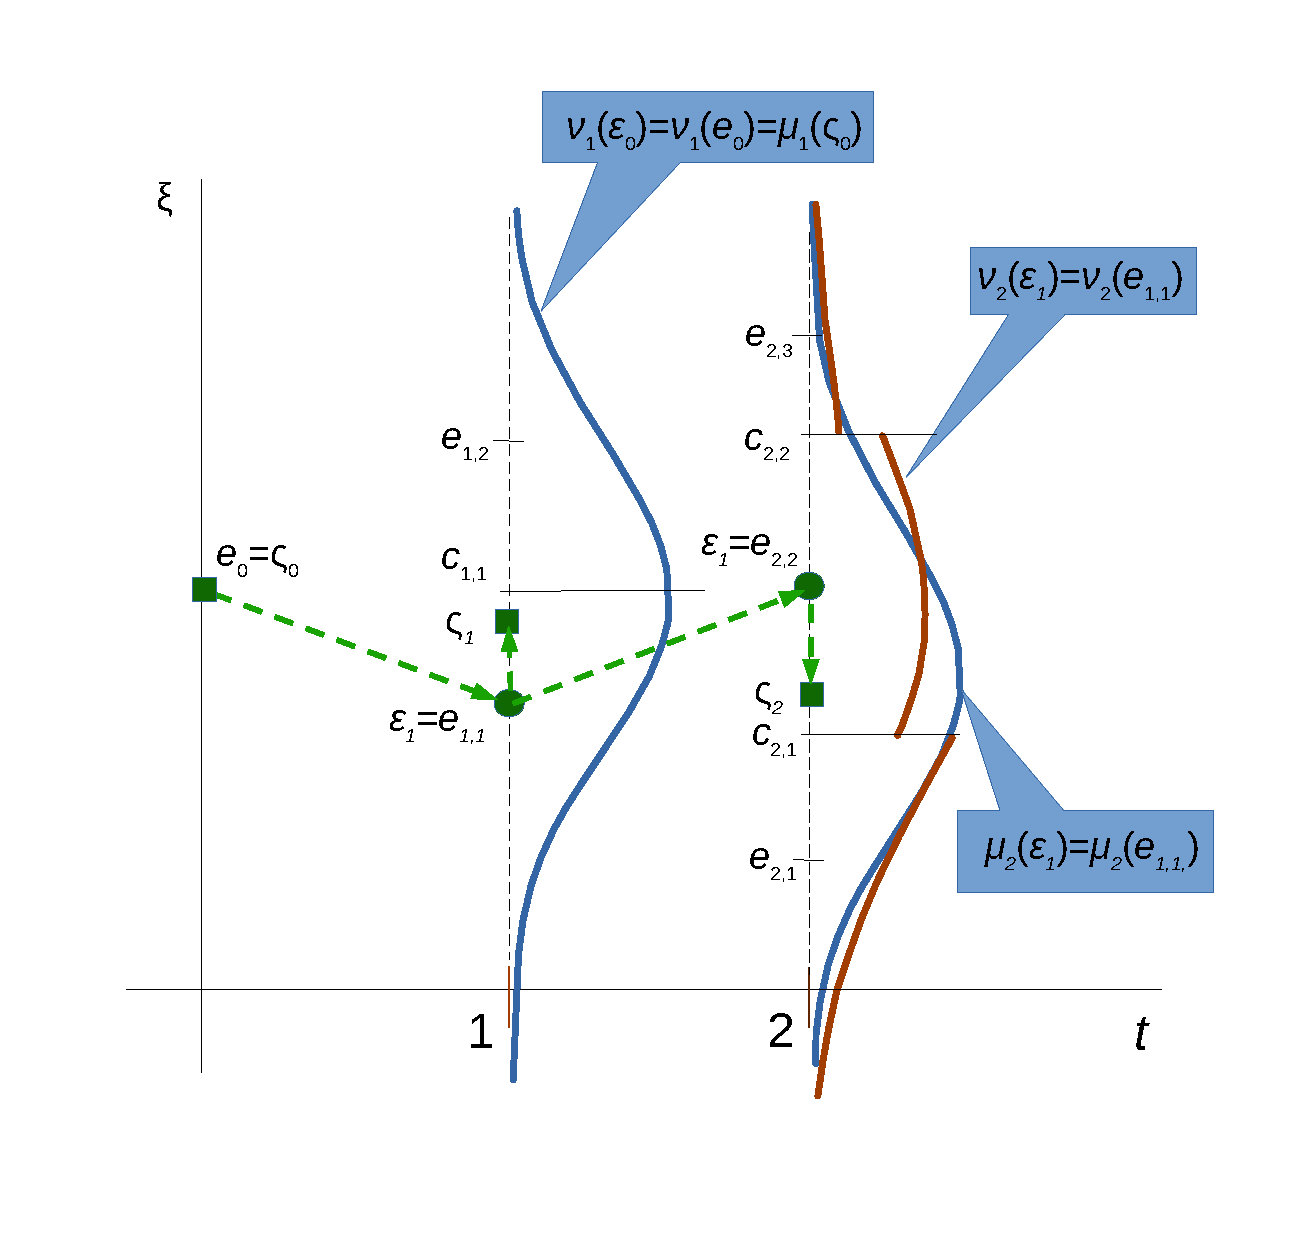
\includegraphics[scale=0.5]{illust}
\caption{Smoothed quantization. Realizations of $\epsilon$: circles, realizations of $\varsigma$: squares, quantized (conditional) distributions: blue, (conditional) distributions of $\varsigma$: orange. Succession of simulation: green arrows.}
\label{fig:ilust1}
\end{center}
\end{figure}


\begin{proposition}
\label{prop:vs}(i) $\varepsilon$ is uniquely defined by $\varsigma$.
In particular, for each $1\leq t\leq T$, 
\[
\varepsilon_{t}=\epsilon_{t}(\varsigma_{t}),\qquad\epsilon_{t}(s)\defined\sum_{i=1}^{k_{t}}e_{t,i}\charf_{C_{t,i}}(s),
\]
(ii) $\varsigma$ is Markov, ruled by distributions 
\[
\nu_{t}(\bullet|s)=\sum_{i=1}^{k_{t}}\omega_{t,i}(\bullet)\mu_{t}(C_{t,i}|\epsilon_{t-1}(s)),\qquad s\in\R^p,\qquad  1\leq t\leq T,
\]
(iii) for each $1\leq t\leq T$, $\nu_{t}(\bullet)$ is constant on any $C_{t-1,i}$, $1\leq i\leq k_{t-1}$; in particular, $\nu_{t}(\varsigma_{t-1})=\nu_{t}(\varepsilon_{t-1})$,\\
(iv) $\xi_{1}\stackrel{d}{=}\varsigma_{1}$ (meaning that the distributions of the left-hand side and the right-hand side agree),\\
(v) $\L(\varsigma)$ does not depend on $e_{T,1},\dots,e_{T,k_T}$.
\end{proposition}

\begin{proof}
(i) is clear.\\
(ii) Denote 
$\iota_{t}\defined i_{t}(\varepsilon_{t})$, $0\leq t\leq T.$
We have
\begin{multline*}
\P[\varsigma_{t}\in\bullet|\overline{\varsigma}_{t-1}]\stackrel{(i)}{=}\P[\varsigma_{t}\in\bullet|\overline{\varsigma}_{t-1},\bareps_{t-1}]=\E(\P[\varsigma_{t}\in\bullet|\overline{\varsigma}_{t-1},\bareps_{t}]|\overline{\varsigma}_{t-1},\bareps_{t-1})
\\
\stackrel{(\ref{eq:vsdef})}{=}\E(\omega_{t,\iota_{t}}(\bullet)|\overline{\varsigma}_{t-1},\bareps_{t-1})
=\sum_{i=1}^{k_{t}}\omega_{t,i}(\bullet)\P[\iota_{t}=i|\overline{\varsigma}_{t-1},\bareps_{t-1}]\\ \stackrel{(\ref{eq:skelet})}{=}
\sum_{i=1}^{k_{t}}\omega_{t,i}(\bullet)\mu(C_{t,i}|\varepsilon_{t-1})
\stackrel{(i)}{=}\nu_{t}(\bullet|\varsigma_{t-1}).
\end{multline*}
(iii) follows from the definition of $\nu_t$ and from (i).\\
(iv) follows by imposing. \\
(v) is clear from (ii). 
\end{proof}
\noindent Definitions (\ref{eq:skelet}) and (\ref{eq:vsdef}) give us instructions how to simulate the process $\varsigma$: at the $t$-th time step, a value of $\epsilon_t$  is drawn from $\theta(\bullet|\epsilon_{t-1})$ first and, consequently, $\varsigma_t$ is 
drawn from $\omega_{t,i_t(\epsilon_t)}$. Alternatively, as the distribution of $\varsigma_t$ depends on the past only through $\epsilon_t$, we can generate the skeleton process first and smooth it afterwards. For better understanding, we graphically illustrate our construction 
by an example with $T=2$, $k_1=2$, and $k_2=3$ in Figure \ref{fig:ilust1}. 

%\tbd{move up} 
Before stating an upper bound of the approximation error, measured
by $\d(\xi,\varsigma)$, assume, without loss of generality, that
\begin{equation}
\xi_{t}=g_{t}(\xi_{t-1},U_{t}),\qquad1\leq t\leq T,\label{eq:xxu}
\end{equation}
where $U_{1},\dots,U_{T}$ are i.i.d. and $g_{1},\dots g_{T}$ measurable (see \cite{Kallenberg02} Proposition
8.6 for the proof that such a representation always exists).

\begin{theorem}
\label{prop:est} Let there exist a measurable
function $h_{t}$ with $\E h_{t}(U_{t})<\infty$ for any $1\leq t\leq T$ such that 
\begin{equation}
\|g_{t}(x,u)-g_{t}(y,u)\|\leq h_{t}(u)\|x-y\|,\qquad
x,y\in\R^{p},\quad u\in\supp(U_{t}).\label{eq:htl}
\end{equation}
Then, for any $1\leq t\leq T,$ 
\begin{eqnarray}
\d(\barxi_{t},\barvs_{t}) & \leq & (1+K_{t})\d(\barxi_{t-1},\barvs_{t-1})+K_{t}\E\|\varsigma_{t-1}-\varepsilon_{t-1}\| \nonumber \\
& & \qquad \qquad +\E\dw(\mu_{t}(\varepsilon_{t-1}),\nu_{t}(\varepsilon_{t-1}))\label{eq:dfirst}\\
 & \leq & \sum_{\tau=1}^{t-1}\kappa_{\tau}\sum_{i=1}^{p}\sum_{j=1}^{k_{\tau}}\int|x-e_{\tau,j}^{i}|q_{\tau,j}\omega^i_{\tau,j}(dx)
\nonumber \\ 
& & \qquad \qquad +\sum_{\tau=2}^{t}\lambda_{\tau}\sum_{i=1}^{k_{\tau-1}}q_{\tau-1,i}\dw(\mu_{\tau}(e_{\text{\ensuremath{\tau}}-1,i}),\nu_{\tau}(e_{\tau-1,i})),\label{eq:dthird}
\end{eqnarray}
where
\[
K_{\tau}=\E h_\tau (U_{\tau}),\qquad1\leq\tau\leq T,
\]
%\begin{equation}
%\tilde{\omega}_{\tau,i,j}=\sum_{k:e_{\tau,k}^{i}=e_{\tau,j}^{i}}q_{\tau,k}\omega_{\tau,k}%^{i},\qquad1\leq j\leq k_{\tau,i},\quad 1\leq i\leq p, \quad 1\leq\tau\leq T-1,
%\label{eq:tomegadef}
%\end{equation}
\[
\kappa_{\tau}=K_{\tau+1}\prod_{i=\tau+2}^{t}(1+K_{i}),\qquad1\leq\tau\leq t-1,
\]
\[
\lambda_{\tau}=\prod_{i=\tau+1}^{t}(1+K_{i}),\qquad2\leq\tau\leq t,
\]
with $\prod_{i=s+1}^{s}x_{i}\defined1;$ here, \textup{\emph{for any
}}\textup{$1\leq\tau\leq t,$} $1\leq k\leq k_{\tau},$$q_{\tau,k}=\P[\varepsilon_{\tau}=e_{\tau,k}],$
and, for any $1\leq i\leq p$,\textup{\emph{ $\omega_{\tau,k}^{i}$
is the $i$-th marginal distribution of $\omega_{\tau,k}$. }}
\end{theorem}

\begin{remark}
(\ref{eq:htl}) holds if\\
(i) $\xi_{t}=C+D\xi_{t-1}+U_{t}$ (with $h_{t}(u)\equiv\|D\|$). \\
(ii) $\xi_{t}=U_{t}\xi{}_{t-1}$ and $\E \| U_t \| < \infty$ (with $h_{t}(u)\equiv\|u\|$).
\end{remark}

%\begin{remark}
%\label{rem:onedim}If $p=1$, then the left hand summand in (\ref{eq:dthird})
%reduces to $\sum_{\tau=1}^{t-1}\kappa_{\tau}\sum_{j=1}^{k_{\tau}}\int|x-e_{\tau,j}|q_{\tau,j}%%
%\omega_{\tau,j}(dx)$.
%\end{remark}


\begin{proof}
As, by Lemma \ref{lem:flemma} in Appendix and (\ref{eq:htl}),
\begin{multline}
\mathrm{d}(\mu_{t}(x),\mu_{t}(y))\leq\int\|g(x,u)-g(y,u)\|\L(U_{t})(du)
\\
\leq\|x-y\|\int h_{t}(u)\L(U_{t})(du)
=K_t \|x-y\| 
,\qquad x,y\in\R^{p},
\label{eq:liplip}
\end{multline}
(\ref{eq:ktl}) holds true. Consequently, by Proposition \ref{prop:pp},
\begin{equation}
\d(\barxi_{t},\barvs_{t})\leq(1+K_{t})\d(\barxi_{t-1},\barvs_{t-1})+\E\mathrm{d}(\mu_{t}(\varsigma_{t-1}),\nu_{t}(\varsigma_{t-1})).
\label{eq:dxixi}
\end{equation}
Using triangular inequality, Proposition \ref{prop:vs} (iii), and (\ref{eq:liplip}), we have
\begin{multline*}
\mathrm{d}(\mu_{t}(\varsigma_{t-1}),\nu_{t}(\varsigma_{t-1}))\leq\mathrm{d}(\mu_{t}(\varsigma_{t-1}),\mu_{t}(\varepsilon_{t-1}))+\mathrm{d}(\mu_{t}(\varepsilon_{t-1}),\nu_{t}(\varepsilon{}_{t-1}))
\\
\leq
K_t \E \|\varsigma_{t-1}-\varepsilon_{t-1}\|+\mathrm{d}(\mu_{t}(\varepsilon_{t-1}),\nu_{t}(\varepsilon{}_{t-1})).
\end{multline*}
Combined with (\ref{eq:dxixi}) we get (\ref{eq:dfirst}). 

Further, by induction, 
using the facts that $\xi_{0}=\varepsilon_{0}$ and that $\d(\barxi_{1},\barvs_{1})=0$
(by Proposition \ref{prop:vs} (iv)), we get
\[
\d(\barxi_{t},\barvs_{t})\leq\sum_{\tau=1}^{t-1}\kappa_{\tau}\E\|\varsigma_{\tau}-\varepsilon_{\tau}\|+\sum_{\tau=2}^{t}\lambda_{\tau}\E\dw(\mu_{\tau}(\varepsilon_{\text{\ensuremath{\tau}}-1}),\nu_{\tau}(\varepsilon_{\tau-1}))
\]
which proves (\ref{eq:dthird}) since 
\[
\E\dw(\mu_{\tau}(\varepsilon_{\text{\ensuremath{\tau}}-1}),\nu_{\tau}(\varepsilon_{\tau-1}))=\sum_{i=1}^{k_{\tau-1}}q_{\tau-1,i}\dw(\mu_{\tau}(e_{\text{\ensuremath{\tau}}-1,i}),\nu_{\tau}(\boldsymbol{e}_{\tau-1,i}))
\]
and  
\begin{multline*}
\E\|\varsigma_{\tau}-\varepsilon_{\tau}\|\stackrel{\text{Prop. \ref{prop:vs} (i)}}{=}\E\|\varsigma_{\tau}-\epsilon_{\tau}(\varsigma_{\tau})\|=\E(\E(\|\varsigma_{\tau}-\epsilon_{\tau}(\varsigma_{\tau})\||\varsigma_{\tau-1}))\\
\stackrel{\text{Prop. \ref{prop:vs} (ii)}}{=}\E(\int\|s-\epsilon_{\tau}(s)\|\nu_{\tau}(ds|\varsigma_{\tau-1}))\stackrel{\text{Prop. \ref{prop:vs} (iii)}}{=}\E(\int\|s-\epsilon_{\tau}(s)\|\nu_{\tau}(ds|\varepsilon_{\tau-1}))\\
=\sum_{k=1}^{k_{\tau-1}}q_{\tau-1,i}\sum_{j=1}^{k_{\tau}}\mu_{\tau}(C_{\tau,j}|e_{\tau-1,k})\int\|s-e_{\tau,j}\|\omega_{\tau,j}(ds)\\
\stackrel{q_{\tau,j}=\sum_{k}q_{\tau-1,k}\mu_{\tau}(C_{\tau,j}|e_{\tau-1,k})}{=}\sum_{j=1}^{k_{\tau}}q_{\tau,j}\int\|s-e_{\tau,j}\|\omega_{\tau,j}(ds)\\
=\sum_{j=1}^{k_{\tau}}q_{\tau,j}\sum_{i=1}^{p}\int|s-e_{\tau,j}^{i}|\omega_{\tau,j}^{i}(ds)=\sum_{i=1}^{p}\sum_{j=1}^{k_{\tau}}\int|s-e_{\tau,j}^{i}|\left(q_{\tau,j}\omega_{\tau,j}^{i}\right)(ds)
%ˇ\\
%=\sum_{i=1}^{p}\sum_{k=1}^{k_{\tau,i}}\int|s-e_{\tau,m}^{i}|\left(\sum_{j:e_{\tau,j}^{i}/%=e_{\tau,k}^{i}}q_{\tau,j}\omega_{\tau,j}^{i}\right)(ds),\qquad1\leq\tau<t.
\end{multline*}
\end{proof}

\noindent The next Theorem provides conditions for convergence of the smoothed quantization
in the one-dimensional case.
\begin{theorem}
\label{thm:conv}Let $p=1$. Assume (\ref{eq:htl}) and let the unconditional distributions  $\tilde{\mu}_{1},\dots,\tilde{\mu}_{t}$
be absolutely continuous such that their tails $$T_\tau(x) \defined \max(\tilde \mu_\tau(-\infty,-x],\tilde \mu_\tau(x,\infty))$$ are $O(x^{-a})$, $\tau=1,\dots,t$,
for some $a>1$. For each $1\leq t\leq T$ and for each covering with representatives
$\C=((C_{1},\dots,C_{k}),(e_{1},\dots,e_{k}))$, denote
\begin{equation}
D_{t}^{\C}(\bullet)\defined\dw(\mu_{t}(\bullet),\theta_{t}(\bullet)),\label{eq:firstlip}
\end{equation}
\begin{equation}
E_{t}^{\C}(\bullet)\defined\sum_{i=2}^{k_{t}-1}\mu_{t}(C_{i}|\bullet)\int|x-e_{t,i}|\omega_{t,i}(dx),\label{eq:seclip}
\end{equation}
\begin{equation}
F_{t}^{\C}(\bullet)\defined\mu_{t}(C_{1}|\bullet),\qquad G_{t}^{\C}(\bullet)\defined\mu_{t}(C_{k}|\bullet),\label{eq:thirdlip}
\end{equation}
and assume that $D^{\C}$, $E^{\C}$, $F^{\C}$, and $G^{\C}$ are Lipschitz (the Lipschitz constants may depend on $\C$). Then there
exists a sequence $\mathfrak{C}_{1},\mathfrak{C}_{2},\dots$ of collections
of coverings such that $\d(\barxi_{T},\barvs_{,T}^{\boldsymbol{\mathfrak{C}_{i}}})\rightarrow0$,
where, for any covering collection $\mathfrak{C},$ $\varsigma^{\mathfrak{C}}$
is the smoothed quantization of $\barxi_{T}$ defined by $\mathfrak{C}$.
\end{theorem}

\begin{proof}
Let $\mathfrak{C}=(\C_{0},\dots,\C_{T})$ be a collection of coverings.
For any $1\leq t\leq T$, let $R_{t}^{\C_{t}}$ and $T_{t}^{\C_{t}}$
be the Lipschitz constants of $D_{t}^{\C_{t}}$, $E_{t}^{\C_{t}}$, respectively
and let $S_{t}^{\C_{t}}$ be the common Lipschitz constant of $F_{t}^{\C_{t}}$
and $G_{t}^{\C_{t}}$. First we show that, for any $1\leq t\leq T$, it holds that
\begin{multline}
\d(\barxi_{t},\barvs_{t}^{\mathfrak{C}})\leq2\dw(\xi_{t},\epsilon_{t}(\xi_{t}))+(1+2K_{t})\d(\barxi_{t-1},\barvs_{t-1}^{\mathfrak{C}})\\
+(R_{t}^{\C_{t}}+S_{t}^{\C_{t}}(\Phi_{t}^{\C_{t}}+\Psi_{t}^{\C_{t}})+T_{t}^{\C_{t}}+K_{t})\d(\barxi_{t-1},\bareps_{t-1}^{\mathfrak{C}})\label{eq:asympb}
\end{multline}
where $\Phi_{t}^{\C_{t}}=\frac{\int_{-\infty}^{c_{t,1}}\tilde{\mu}_{t}(-\infty,x]dx}{\tilde{\mu}_{t}(-\infty,c_{t,1}]}$,
$\Psi_{t}^{\C_{t}}=\frac{\int_{c_{t,k_{t}-1}}^{\infty}\tilde{\mu}_{t}(x,\infty)dx}{\tilde{\mu}_{t}(c_{t,k_{t}-1},\infty)}$,
and it holds that 
\begin{equation}
\d(\barxi_{t},\overline{\varepsilon}_{t}^{\mathfrak{C}})\leq\dw(\xi_{t},\epsilon_{t}(\xi_{t}))+(K_{t}+R_{t}^{\C_{t}}+1)\d(\barxi_{t-1},\overline{\varepsilon}_{t-1}^{\mathfrak{C}}),\label{eq:secondih}
\end{equation}
where $\varepsilon^{\mathfrak{C}}$ the skeleton process defined
by $\mathfrak{C}$. To this end, fix $\mathfrak{C}$ and agree to omit the superscripts indicating
the coverings. We prove (\ref{eq:asympb}) and (\ref{eq:secondih})
simultaneously by induction. 

Clearly, (\ref{eq:asympb}) and (\ref{eq:secondih}) hold for $t=1$
(by Proposition \ref{prop:vs} (iv)).

Let $t>1$ and assume (\ref{eq:asympb}) and (\ref{eq:secondih})
to hold for $t-1$.
By the Lipchitz property of $D_t$, Proposition \ref{prop:thesis} and Kantorovich-Rubinstein Theorem (implying that $\E\|x-y\| \leq \dw(x,y)$ for any $x,y$ with $\E\|x\|+\E\|y\|<\infty$,
\cite{pflug2014multistage} Theorem 2.29), 
\begin{multline}
%\E\dw(\mu_t(\varepsilon_{t-1}),\theta_t(\varepsilon_{t-1})))
%´=
\E D_{t}(\varepsilon_{t-1})
\leq
\underbrace{\E D_{t}(\xi_{t-1})}_
{{=\E\dw(\mu_t(\xi_{t-1}),\theta_t(\xi_{t-1}))
\atop
=
\E(\E\|\xi_{t}-\epsilon_t(\xi_{t})\| |\xi_{t-1}))}
\atop
{=\E\|\xi_{t}-\epsilon_t(\xi_{t})\|=
\dw(\xi_t,\epsilon_t(\xi_t))}}
+
R_t \E\|\xi_{t-1}-\varepsilon_{t-1}\|
\\
\leq \dw(\xi_t,\epsilon_t(\xi_t))+R_{t}\dw(\xi_{t-1},\varepsilon_{t-1}).
\label{eq:mutheta}
\end{multline}
Further, by Proposition \ref{prop:thesis} (note that $\theta_{t}(\varepsilon_{t-1})$
is the quantization of $\nu_{t}(\varepsilon_{t-1})$), the Lipschitz properties and the K-R
Theorem again, we get
\begin{multline}
\E(\dw(\nu_{t}(\varepsilon_{t-1}),\theta_{t}(\varepsilon_{t-1})))
\stackrel{\text{Prop. \ref{prop:thesis}}}
=\E(\sum_{i=1}^{k_{t}}\mu_{t}(C_{t,i}|\varepsilon_{t-1})\int|x-e_{t,i}|\omega_{t,i}(dx))\\
=\Phi_{t}\E F_{t}(\varepsilon_{t-1})+\E E_{t}(\varepsilon_{t-1})+\Psi_{t}\E G_{t}(\varepsilon_{t-1})
\\
\leq\underbrace{\Phi_{t}\E F_{t}(\xi_{t-1})+\E E_{t}(\xi_{t-1})+\Psi_{t}\E G_{t}(\xi_{t-1})}_{=\dw(\xi_{t},\epsilon_{t}(\xi_{t}))}+U_{t}\dw(\xi_{t-1},\varepsilon_{t-1}),\\
U_{t}=S_{t}(\Phi_{t}+\Psi_{t})+T_{t}.\label{eq:efe}
\end{multline}
Thus,
\begin{multline*}
\d(\barxi_{t},\barvs_{t})
\stackrel{\text{(\ref{eq:dfirst}), Prop. \ref{prop:thesis}}}
\leq
(1+K_{t})\d(\barxi_{t-1},\barvs_{t-1})+K_{t}\dw(\varsigma_{t-1},\varepsilon_{t-1})+\E\dw(\mu_{t}(\varepsilon_{t-1}),\nu_{t}(\varepsilon_{t-1}))\\
\stackrel{\text{triang. ineq.}}
\leq
(1+K_{t})\d(\barxi_{t-1},\barvs_{t-1})+K_{t}(\dw(\xi_{t-1},\varsigma_{t-1})+\dw(\xi_{t-1},\varepsilon_{t-1}))\\
+
\underbrace
{\E\dw(\mu_{t}(\varepsilon_{t-1}),\theta_{t}(\varepsilon_{t-1}))}
_{\qquad\qquad \stackrel{(\ref{eq:mutheta})}\leq \dw(\xi_t,\epsilon_t(\xi_t))+ R_{t}\dw(\xi_{t-1},\varepsilon_{t-1})}
+
\underbrace
{\E\dw(\nu_{t}(\varepsilon_{t-1}),\theta_{t}(\varepsilon_{t-1})))}
_
{\qquad\qquad\stackrel{(\ref{eq:efe})}\leq \dw(\xi_t,\epsilon_t(\xi_t))+ U_{t}\dw(\xi_{t-1},\varepsilon_{t-1})},
\end{multline*}
giving (\ref{eq:asympb}) by Lemma \ref{lem:ddd} in Appendix. 

The proof of (\ref{eq:secondih}) is simpler, based on the fact that
\[
\d(\barxi_{t-1},\bareps_{t-1})\leq(1+K_{t})\d(\barxi_{t-1},\bareps_{t-1})+\E\dw(\mu_{t}(\varepsilon_{t-1}),\theta_{t}(\boldsymbol{\varepsilon}_{t-1})),
\]
which may be proved analogously to (\ref{eq:dfirst}) of Theorem \ref{prop:est} and
implies (\ref{eq:secondih}) by (\ref{eq:mutheta}) and Lemma
\ref{lem:ddd} in Appendix.

Therefore, both (\ref{eq:asympb}) and (\ref{eq:secondih}) are proved.

Next we show that, for each $1\leq t\leq T$, there exist a series
of covering collections $\mathfrak{C}_{1},\mathfrak{C}_{2},\dots$
such that 
\begin{equation}
\d(\barxi_{t},\barvs_{t}^{\mathfrak{C}_{n}})\rightarrow0,\qquad \d(\barxi_{t},\bareps_{t}^{\mathfrak{C}_{n}})\rightarrow0.\label{eq:dxde}
\end{equation}
 Clearly, (\ref{eq:dxde}) with $t=T$ proves the Theorem. We shall proceed by induction while  for $t=0$, (\ref{eq:dxde}) holds trivially. 

Let $t>0$ and assume (\ref{eq:dxde}) to hold for $t-1$, i.e. that there
exists a sequence $\mathfrak{D}_{1},\mathfrak{D}_{2},\dots$ of covering
collections such that (\ref{eq:dxde}) holds for $t-1$ and $\mathfrak{D_{\bullet}}$ instead of
$t$ and $\mathfrak{C_{\bullet}}$. 


First, let $\C_{i}=(\{C_{1}^{i},\dots,C_{k_{i}}^{i}\},\{e_{1}^{i},\dots,e_{k_{i}}^{i}\}),$$i\in\N$,
be coverings such that $\lim_{i}\dw(\xi_{t},\epsilon_{i,t}(\xi_{t}))\rightarrow0$
where $\epsilon_{i,t}(\bullet)=\sum_{j}e_{j}^{i}\charf_{C_{j}^{i}}(\bullet)$: their existence is guaranteed by \cite{Smid09c}, Theorem 1. For
each $n\in\N$, let $i(n)$ be such that $\dw(\xi_{t},\epsilon_{i(n),t}(\xi_{t}))\leq\frac{1}{4n}$.

Next, for any $n\in \N$ and any covering $\C$, put 
\begin{equation}
\delta_{n}^{\C}=(1+2K_{t})\dw(\barxi_{t-1},\barvs_{t-1}^{\mathfrak{D}_{n}})
+(K_{t}+R_{t}^{\C}+\max(1,S_{t}^{\C}(\Phi_{t}^{\C}+\Psi_{t}^{\C})+T_{t}^{\C}))\dw(\barxi_{t-1},\bareps_{t-1}^{\mathfrak{D}_{n}})\label{eq:deltac}
\end{equation}
and note that $\delta_{n}^{\C}\rightarrow0$ by the induction hypothesis. 
For each $i,n\in\N$, let $j(i,n)$ be such that $\delta_{j(i,n)}^{\C_{i}}\leq\frac{1}{2n}$.

Finally, for any $n$, put $\mathfrak{C}_{n}=(\mathfrak{D}_{j(i(n),n)},\C_{i(n)})$.
By imposing into (\ref{eq:asympb}), we get 
\begin{equation}
\d(\barxi_{t},\barvs_{t}^{\mathfrak{C}_{n}})\leq2\dw(\xi_{t},\epsilon_{i(n),t}(\xi_{t}))+\delta_{j(i(n),n)}^{\C_{i(n)}}\leq\frac{1}{n}.
\label{eq:dbx}
\end{equation}
Similarly we get, using (\ref{eq:secondih}), that $\d(\barxi_{t},\bareps_{t}^{\mathfrak{C}_{n}})\leq\frac{1}{n}$,
which together with (\ref{eq:dbx}) proves (\ref{eq:dxde}).
\end{proof}
\noindent The next Proposition states sufficient conditions for (\ref{eq:firstlip})-(\ref{eq:thirdlip}).
\begin{proposition}
\label{lem:dif}Let $p=1$ and, for each $1\leq t\leq T$, let 
\[
G_{t}(x|y)\defined\mu_{t}((-\infty,x]|y)
\]
be differentiable in both $x$ and $y$ such that, for each $x$ and $y$,
\[
\left|\frac{\partial}{\partial y}G_{t}(x|y)\right|\leq h(x,y)
\]
for some unimodal $h(\bullet,y)$ with $\int h(x,\bullet)dx$ and
$\max_{x}h(x,\bullet)$ uniformly bounded. Let 
$$\frac{\partial}{\partial y}\int_{-\infty}^{c}G_{t}(x|y)dx=\int_{-\infty}^{c}\frac{\partial}{\partial y}G_{t}(x|y)dx$$
and 
$$\frac{\partial}{\partial y}\int_{c}^{\infty}[1-G_{t}(x|y)]dx=-\int_{c}^{\infty}\frac{\partial}{\partial y}G_{t}(x|y)dx$$
for any $c\in\R$. Then the Lipschitz properties of (\ref{eq:firstlip})-(\ref{eq:thirdlip})
hold true. 
\end{proposition}

\begin{proof}
Fix $1\leq t\leq T$ and a covering $\C$ and agree to omit corresponding
indexes. Let $y\in\R.$ By \cite{Vallander73} (or perhaps \cite{Pflug01}), we have
\[
D(y)=I_{0}(y)+\dots+I_{k}(y),
\]
where
\[
I_{0}(y)=\int_{-\infty}^{e_{1}}G(x|y)dx,\qquad I_{k}(y)=\int_{e_{k}}^{\infty}[1-G(x|y)]dx,
\]
\[
I_{i}(y)=\int_{e_{i}}^{c_{i}}[G(c_{i}|y)-G(x|y)]dx+\int_{c_{i}}^{e_{i+1}}[G(x|y)-G(c_{i}|y)]dx,
\qquad 1\leq i\leq k-1.
\]
Denoting $g(\bullet|y)=\frac{\partial}{\partial y}G(\bullet|y)$,
we get
\[
I'_{0}(y)=\int_{-\infty}^{e_{1}}g(x|y)dx,\qquad I'_{k}(y)=-\int_{e_{k}}^{\infty}g(x|y)dx,
\]
\begin{multline*}
I_{i}'(y)=-\int_{e_{i}}^{c_{i}}g(x|y)dx+\int_{c_{i}}^{e_{i+1}}g(x|y)dx+[(c_{i}-e_{i})-(e_{i+1}-c_{i})]g(c_{i}|y),\\ 
\qquad 
1\leq i\leq k-1,
\end{multline*}
so
\begin{multline}
\left|\frac{\partial}{\partial y}D(y)\right|
\leq\text{\ensuremath{\int_{-\infty}^\infty|g(x|y)|dx+
\sum_{i=1}^{k-1}((c_{i}-e_{i})+(e_{i+1}-c_{i}))}}|g(c_{i}|y)|\\
\leq\int h(x,y)dx+2\sum_{i=1}^{k-1}|e_{i+1}-e_{i}||h(c_{i},y)|\leq\int h(x,y)dx+2\int h^{*}(x,y)dx,\\
h^{*}(x,y)=\begin{cases}
h(x+\hat e,y) & x<m-\hat{e}\\
\max h(\bullet,y) & m-\hat{e}\leq x\leq m+\hat{e}\\
h(x-\hat{e},y) & x>m+\hat{e}
\end{cases}\label{eq:ddy}
\end{multline}
where $m$ is the mode of $h(\bullet,y)$ and $\hat e = \max_{i=1,\dots,k-1} |e_{i+1}-e_i|$ (we have used the fact that $h(\bullet,y)$ is non-decreasing up to $m$ and non-increasing from $m$). Clearly, $\int h^{\star}(x,y)dx\leq\int h(x,y)dx+2\hat{e}\max h(\bullet,y)$
which, together with (\ref{eq:ddy}), proves (\ref{eq:firstlip})
as both $\int h(x,y)dx$ and $\max h(\bullet,y)$ are uniformly bounded, hence
the derivative is uniformly bounded and the Lipschitz property of $D$ holds. 

As for (\ref{eq:seclip}), we have

\begin{multline*}
E(y)=G(c_{1}|y)\int_{e_{1}}^{c_{1}}(x-e_{1})\omega_{1}(dx)
+\sum_{i=2}^{k-1}(G(c_{i}|y)-G(c_{i-1}|y))\int_{c_{i-1}}^{c_{i}}|x-e_{i}|\omega_{i}(dx)\\
+(1-G(c_{k}|y))\int_{c_{k-1}}^{e_{k}}(e_{k}-x)\omega_{k}(dx)
\end{multline*}
so 
\begin{multline*}
\left|\frac{\partial}{\partial y}E(y)\right|
%=\left|g(c_{1}|y)\int_{e_{1}}^{c_{1}}(x-e_{1})\omega_{1}(dx)+\right.\\
%\left.
%\sum_{i=2}^{k-1}(g(c_{i}|y)-g(c_{i-1}|y))\int_{c_{i-1}}^{c_{i}}|x-e_{i}|\omega_{i}(dx)-g(c_{k-1}|%y)\int_{c_{k-1}}^{e_{k}}(e_{k}-x)\omega_{k}(dx) 
%\right|
%ˇ\\
\leq h(c_{1},y)\int_{e_{1}}^{c_{1}}(c_{1}-e_{1})F_{1}(dx)+\sum_{i=2}^{k-1}(h(c_{i},y)+h(c_{i-1},y))\int_{c_{i-1}}^{c_{i}}(c_{i}-c_{i-1})\omega_{i}(dx)\\
+h(c_{k-1},y)\int_{c_{k-1}}^{e_{k}}(e_{k}-c_{k-1})\omega_{k}(dx)\\
\leq h(c_{1},y)(c_{1}-e_{1})+\sum_{i=2}^{k-1}(h(c_{i},y)+h(c_{i-1},y))(c{}_{i}-c_{i-1})+h(c_{k-1},y)(e_{k}-c_{k-1})
\end{multline*}
which gives the Lipschitz property of  (\ref{eq:seclip}) by applying a similar trick as in the
case of $D$ to the middle term. 

Finally, as $h$ is uniformly bounded, so is the derivative of $G$
and the Lipschitz property of (\ref{eq:thirdlip}) holds.
\end{proof}

\begin{example}
Let $p=1$ and let $\xi_{t}$ be AR(1), i.e. $\xi_{t}=a\xi_{t-1}+\epsilon_{t}$,
$1\leq t\leq T,$ where the c.d.f. $F$ of $\text{\ensuremath{\epsilon_{t}}}$
is differentiable with $F'=f$ unimodal. Then 
\[
G_{t}(x|y)=F(x-ay),\qquad\frac{\partial}{\partial y}G_{t}(x|y)=-af(x-ay),
\]
so we may choose $h(x,y)=|a|f(x-ay)$, giving $\int h(x,y)=a$, $\max h=|a|\max f$.\footnote{The change-of-derivative condition is met as 
$$
\frac{\partial}{\partial y}\int_{-\infty}^{c}F(x-ay)dx=\frac{\partial}{\partial y}\int_{-\infty}^{c-ay}F(z)dz
=-aF(c-ay)=-a\int_{-\infty}^{c-ay}f(z)dz=-a\int_{-\infty}^{c}f(x-ay)dx
$$
and similarly for the upper tail.} Thus, by Proposition \ref{lem:dif}, the Lipschitz properties of (\ref{eq:firstlip})-(\ref{eq:thirdlip})
hold and, consequently, Theorem \ref{thm:conv} holds once the tails
of each $\sum_{\tau=1}^{t}a^{t-\tau}\epsilon_{t}$, $1\leq t\leq T,$
are \emph{$O(x^{-\alpha})$ }for some \emph{$\alpha>1$}, which is
the true in most cases because the converse would imply infinite second
moments. 
\end{example}

\begin{example}
If $\xi_{t}=\xi_{t-1}\epsilon_{t}$ then $G_{t}(x|y)=\P[\epsilon_{t}\leq\frac{x}{y}]=F(\frac{x}{y})$
where $F$ is the c.d.f. of $\epsilon_{t}$. Here, unfortunately,
Proposition \ref{lem:dif} cannot be used because $\int\frac{\partial}{\partial y}G_{t}(x|y)dx=-\frac{1}{y^{2}}\int F'(\frac{x}{y})dx=-\frac{1}{y}$
is unbounded. Certainly, we can assume $\xi_{t}$ to be a random walk
and modify the mappings $\phi_{t},\psi_{t}$ and $\Xi_{t}$ in (\ref{eq:exi})
(i.e. use $\phi_{t}(e^{x},u)$ instead of $\phi_{t}(x,u)$ etc.);
however it is not guaranteed that the nested distance of the exponentials
would converge, too. 
\end{example}

\begin{remark}
A version of Theorem \ref{thm:conv} for $p>1$ can be formulated
for the price of more complex notation; however, a counterpart of (\ref{eq:seclip}) seems impossible to be verified even
for the autoregression as the probabilities $q_{\bullet}$ are involved. 
\end{remark}

\noindent Finally, we prove that the nested distance does not increase when
we consider the i.i.d. part of the underlying process, which is not approximated.
\begin{proposition}
\label{prop:witheta}Let $\eta$ be a process taking values in $\R^{q}$
with $\eta_{0}$ deterministic, such that $\xi\indep{\eta}$ and $\varsigma\indep{\eta}$, where $\indep$ means independence.
Then $\d((\xi,\eta),(\varsigma,\eta))\le\d(\xi,\varsigma)$.
\end{proposition}

\begin{proof}
See Lemma \ref{lem:indep} in Appendix. 
\end{proof}


\section{\label{sec:approx}Approximation of the Multistage Problem}

%Let the Markov random parameter $\xi$ of Problem (\ref{eq:p}) have
%absolutely continuous marginal distributions. 
The question we deal
with in the present Section is the choice of a (rectangular) covering
collection $\mathfrak{C}=(\C_{1},\dots,\C_{T})$ so that the smoothed
quantization $\varsigma$ of $\xi,$ defined by $\mathfrak{C}$ is
suitable and as exact as possible.

The first thing to be taken into account is computability. Within the plain SDDP, $T-1$ collections of cuts, approximating
the cost-to-go functions, are maintained, and each of these collections
is updated during each backward pass, while, in our implementation of Markov SDDP, the number
of the cut collections equals to $\kappa=\sum_{t=1}^{T}k_{t}=\sum_{t=1}^{T}\prod_{i=1}^{p}k_{t,i}$
(the total number of the skeleton processes atoms) and, during each
backward pass, only one collection per stage is updated. Therefore,
it could be expected that the time complexity of the solution will
be roughly linear in $\kappa$. Taking into account that a solution of a single problem by the plain
SDDP takes tens of minutes on a regular PC (with processor Intel Core 5 and 16 GB RAM), it is clear that the numbers $k_{t,i}$ cannot be
high, especially given multi-dimensional $\xi_{t}$, and even
in the one-dimensional it would be very time consuming to exploit the
asymptotic properties we proved. In any case, the number of the atoms
is limited by our computational resources.

Having determined the numbers of the atoms we can computationally afford, the next step is to choose the
frontiers of the covering sets and the representatives. As we have
already premised, we find reasonable to choose these parameters so
that $\d(\xi,\varsigma)$ (hence $\d((\xi,\eta),(\varsigma,\eta))$
by Proposition \ref{prop:witheta}) is minimized. 
Unfortunately, such minimization is a very complex task, even if we resort to the minimization of the upper bound (\ref{eq:dthird}).
That said, finding optimal representatives with respect to (\ref{eq:dthird})
with the frontiers known is a complex, possibly non-convex problem:
the second part of (\ref{eq:dthird}) and the dependence between
the stages being due. However, if we believe that the distributions
$\omega_{t,i}(\bullet|e)$ approximate the normalized versions of
$\mu_{t}(\bullet\cap C_{t,i}|e)$ well, then we can regard the second part of (\ref{eq:dthird}) less critical and concentrate on the
first part; contrary to the whole expression, finding the optimal
representatives (with the frontiers known) is easy here as we minimize a sum of terms 
$$
\sum_{j=1}^{k_{\tau}}\int|x-e_{\tau,j}^{i}|q_{\tau,j}\omega^i_{\tau,j}(dx)
=
\sum_{k=1}^{k_{\tau,i}} \int|x-e_{\tau,i,k}| \left(\sum_{j:e^i_{\tau,j}=e_{\tau,i,k}} q_{\tau,i,k} \right)
\omega^i_{\tau,k} (dx)
$$
where $e_{\tau,i,1},\dots e_{\tau,i,k_{\tau,i}}$ are the possible values of $e^i_{\tau,\bullet}$. It is well known, that (each summand on the) right hand side is minimized by $e_{t,i}^{i}=\mathrm{median}(\omega^i_{t,j})$.
% https://groups.google.com/forum/#!topic/sci.math.stat/1HuyzpvMXbw

Unfortunately, as we have premised, not all $\varsigma$'s with a reasonable nested distance
are suitable for the approximation of Problem (\ref{eq:p}). In particular,
it may happen that, unlike the original problem, the approximate
version is unbounded. To illustrate this, consider a (hypothetical)
asset-liability problem in which it is necessary to satisfy a random 
liability, no greater than some constant $b$, at the time $T$ by means of buying an asset at the times
$0,\dots,T-1$. Say that the decision criterion is a nested mean-CVaR and that, in-line with Efficient Market Hypothesis (see \cite{Cuthbertson97}), the asset prices are martingale (see \cite{Kallenberg02}, Chapter 7). Given these assumptions, there is no reason to buy more assets than $b$, because buying more than $b$ assets up to $T-1$ and selling them at $T$ would (possibly) increase
risk (CVaR in our case) without increasing mean. However, as our approximation uses ``incorrect'' conditioning value, it can happen that, despite the true price process is a martingale, the approximated one is a sub-martingale, i.e. the prices increase on average (to see it, recall that $\E(\varsigma_{t+1}|\varsigma_t=\bullet)$
is piece-wise constant by Proposition \ref{eq:dthird} (iii), so $\E(\varsigma_{t+1}|\varsigma_{t})\neq\varsigma_{t}$
almost surely once $\omega$'s are absolutely continuous). If this (false) increase is high enough and/or the risk aversion is small enough, then, within the approximating problem, it could be ``reasonable'' to buy unlimited amounts of the asset to sell it at $T$. As a result, these (false) arbitrage opportunities can completely overshadow the asset-liability
management since the profits from the ``speculation'' would be unlimited. Clearly, to avoid this problem, the approximation has to be modified.

Proceeding generally, we start by giving a simple criterion, which,
if fulfilled, guarantees boundedness of $\rho$ in Problem (\ref{eq:p})
from below, which, among other things, precludes arbitrage.

\begin{proposition}
\label{cor:feas} Let there exist integrable random functions $f_{t}:\R^{d_{t}}\rightarrow\R$, $f_t \in \F_t$,
$0\leq t<T$, and a constant $\gamma$ such that, for each feasible
policy $x$, 
\begin{equation}\label{eq:f1}
\sigma_T(c'{}_{T}x_{T})\geq f_{T-1}(x_{T-1})
\end{equation}
\begin{equation}\label{eq:f2}
\sigma_t(c'{}_{t}x_{t}+f_{t}(x_{t}))\geq f_{t-1}(x_{t-1}),\qquad1\leq t< T,
\end{equation}
\begin{equation}\label{eq:f3}
c'_{0}x_{0}+f_{0}(x_{0})\geq\gamma.
\end{equation}
Then the optimal value of (\ref{eq:p}) is bounded from below by $\gamma$.

\end{proposition}

\begin{proof} Follows easily by gradual application of (\ref{eq:f1}) \dots (\ref{eq:f3}) to the criterion of Problem (\ref{eq:p}).
%\begin{multline*}
%\rho(c'_{0}x_{0},\dots,c'_{T}x_{T})\geq\\
%\geq c'_{0}x_{0}+\E(\dots\E(c'_{T-2}x_{T-2}+\E(c_{T-1}x_{T-1}+\E(c'_{T}x_{T}|\F_{T-1})|\F_{T-2})|%%\F_{T-3})\dots)\\
%\geq c'_{0}x_{0}+\E(\dots\E(c'_{T-2}x_{T-2}+\E(c_{T-1}x_{T-1}+f_{T-1}(x_{T-1})|\F_{T-2})|\F_{T-3})%\dots)+\E h_{T-1}\\
%\geq c'_{0}x_{0}+\E(\dots\E(c'_{T-2}x_{T-2}+f_{T-2}(x_{T-2})|\F_{T-3})\dots)
%+\E h_{T-2}+\E h_{T-1}
%\\
%\geq\dots\geq c'_{0}x_{0}+f_{0}(x_{0})+\sum_{\tau=0}^{T-1}\E h_{\tau}\geq h.
%ˇ\end{multline*}
\end{proof}

\begin{corollary}\label{cor:feas}
Let $\sigma_{t}(z|\F_{t-1})\geq \E(z|\F_{t-1})$ for any $\F_t$-measurable random variable $z$ and any $1\leq t\leq T$ and 
let (\ref{eq:f1})-(\ref{eq:f3}) hold with $\E(\bullet|\F_{t-1})$ in place of $\sigma_t(\bullet)$ for any $t$. Then the optimal value of (\ref{eq:p}) is bounded from below by $\gamma$.
\end{corollary}

\begin{proof}Follows from the fact that
\begin{multline*}
\rho(c'_{0}x_{0},\dots,c'_{T}x_{T})
\\ 
\geq c'_{0}x_{0}+\E(\dots\E(c'_{T-2}x_{T-2}+\E(c_{T-1}x_{T-1}+\E(c'_{T}x_{T}|\F_{T-1})|\F_{T-2})|\F_{T-3})\dots).
\end{multline*}

\end{proof}


\begin{remark} The mean-CVaR risk mapping fulfills the assumptions of Corollary \ref{cor:feas}. Indeed, as CVaR is the mean of the right tail distribution (see \cite{rockafellar2002conditional}), which is easy
to show to first-order stochastically dominate the one from which
it is computed, we have $\mathrm{CVaR}(z|\F) \geq \E(z|\F)$ and, consequently,  $\text{mean-CVaR}(z|\F)\geq\E(z|\F)$ for any $z$ and $\F$.
\end{remark}

\noindent The way of finding an approximation $\varsigma$ such that the boundedness
criterion is met clearly depends on the structure of the approximated problem.
As we will see in the next Section, one of the conditions, guaranteeing
the boundedness of the Problem (\ref{eq:p}) with $p=1$, could be

\begin{equation}
\varrho\E(\xi_{t}|\xi_{t-1})\leq\xi_{t-1},\qquad1\leq t\leq T,\label{eq:ref}
\end{equation}
where $\varrho$ is a discount factor. 
Now say that we have a smoothed quantization
$\varsigma$ for which (\ref{eq:ref}) does not hold and we look for a refined
Markov approximation $\chi$ fulfilling (\ref{eq:ref}) which
is ``similar'' to $\varsigma$ in the sense that it is ruled by
conditional probabilities $\varpi_{1},\dots,\varpi_{T}$ such that, for any  $1\leq t \leq T$ and $1\leq i \leq k_{t-1}$,
\begin{itemize}
\item[(i)] $\varpi_{t}(\bullet)$ is constant on $C_{t-1,i}$,
\item[(ii)] $\varpi_{t}(\bullet|e_{t-1,i})=\sum_{j}\pi_{t,i,j}\omega'_{t,j}(\bullet)$ for some discrete distribution
$\pi_{t,i,\bullet}$,
\end{itemize}
where, for any $j$, $\omega'_{t,j}$ is a distribution with $\supp(\omega'_{t,j})\subseteq C_{t,j}$.  It may be easily seen that such a
process fulfills (\ref{eq:ref}) if
\begin{equation}
\varrho\sum_{j}\pi_{t,i,j}\E\omega'_{t,j}\leq d_{t-1,i-1},\qquad1\leq i\leq k_{t-1},1<t<T,\label{eq:refneeded}
\end{equation}
where, for any $\tau$, $d_{\tau,0}=\inf(\supp(\omega'_{\tau,1}))$ and $d_{\tau,j}=c_{\tau,j},1<j\leq k_{\tau}.$

One way to guarantee that such $\chi$ is close to $\varsigma$, for each $2\leq t \leq T$ and $1\leq i \leq k_{t-1}$, is to find $\pi_{t.i,1},\dots,\pi_{t,i,k_{t}}$  so that $\dw(\theta_{t}(e_{t-1,i}),\vartheta_{t,i})$
is minimal, where $\vartheta_{t,i}$ is the distribution with atoms
$e_{t,1},\dots,e_{t,k_{t}}$ and corresponding probabilities $\pi_{t,i,1},\dots,\pi_{t,i,k_{t}}$,
i.e., for each $i$ and $t$, to solve the transportation problem 
\begin{align}
\min_{\pi_{j}\geq0,r_{j,k}\geq0,1\leq j,k\leq k_{t}} & \sum_{j=1}^{k_{t}}\sum_{k=1}^{k_{t}}|e_{t,j}-e_{t,k}|r_{j,k}\label{eq:dwprob}\\
\text{s.t.} & \sum_{j=1}^{k_{t}}r_{j,k}=\mu_{t}(C_{t,k}^{k}|e_{t-1,i}),\qquad1\leq k\leq k_{t}\nonumber \\
 & d_{t-1,i-1}\geq\varrho\sum_{j=1}^{k_{t}}\pi_{j}\E\omega'_{t,i},\qquad \pi_{j}=\sum_{k=1}^{k_{t}}r_{j,k},\qquad1\leq j\leq k_{t}\text{ }\label{eq:cct}
\end{align}
and set $\pi_{t,i,j}=\hat \pi_j$, $1\leq j \leq k_t$, where $\hat \pi_1,\dots, \hat \pi_{k_t}$ is the optimal solution of Problem (\ref{eq:dwprob}). Note that this does not have to be done for $t=1$ as the approximation is perfect here. For all the Problems (\ref{eq:dwprob}) to be feasible,
it should hold 
\begin{equation}
d_{t-1,0}\geq\varrho\E\omega'_{t,1},\qquad2\leq t\leq T\label{eq:cqo}
\end{equation}
because otherwise no combination of $\pi_{1},\dots,\pi_{k_{t}}$
would exist satisfying (\ref{eq:cct}). To
guarantee (\ref{eq:cqo}), we may set
\begin{equation}
\omega'{}_{t,1}=\delta_{e_{t,1}},\qquad \omega'{}_{t,i}=\omega_{t.i},\qquad1<i\leq k_{t},\quad 1\leq t<T,\label{eq:dee}
\end{equation}
which implies (\ref{eq:cqo}) given that 
\begin{equation}
e_{0,1}\geq\varrho e_{1,1}\geq\dots\geq\varrho^{T}e_{1,T}.\label{eq:eeeee}
\end{equation}
In order to have $\chi$ as similar as possible to $\varsigma,$ we
may set $c_{t,1}$ so that $\P[\xi_{t}\leq c_{t,1}]$ is negligible
for each $1\leq t\leq T$.

Finally, we summarize our approximation algorithm:

\bigskip 

{\bf Algorithm 1}

\bigskip

\begin{tabular}{r|l}
1. &  Determine suitable rectangular sets $(C_{t,i})_{1\leq i\leq k_{t}1\leq,t\leq T}$

\\ 2. & For each $t=1$ to $T-1$

\\ 3. &$\qquad$For each $i=1$ to $p$

\\ 4. &$\qquad$$\qquad$For each $j=1$ to $k_{t,i}$

\\ 5. &$\qquad$$\qquad$$\qquad$Put $e_{t,i}^{j}=\mathrm{median}({\omega}^i_{t,j})$  


\\ 6. &$\qquad$$\qquad$End For

\\ 7. &$\qquad$End For

\\ 8. &End For

\\ 9. &Construct the smoothed quantization $\varsigma$ of $\xi$ defined by $C_\bullet$ and $e_\bullet$.

\\ 10. &If $\varsigma$ is suitable
	
\\ 11. &$\qquad$Solve Problem (\ref{eq:p}) with $\varsigma$ instead of $\xi$

\\ 12. &Else 

\\ 13. &$\qquad$Refine $\varsigma$ to get a suitable approximation $\chi$ 

\\ 14. &$\qquad$Solve Problem (\ref{eq:p}) with $\chi$ instead of $\xi$ 

\\ 15. &End If
\end{tabular}

\bigskip 

\noindent When $p=1$, a procedure constructing $\chi$ fulfilling the suitability condition (\ref{eq:ref}) with  $\varrho<1$ may be as follows

\bigskip 

{\bf Algorithm 2}

\bigskip


\begin{tabular}{r|l}
1. & Let $c$ be such that $\P[\xi_t\leq c]$ is small for each $1\leq t\leq T$

\\ 2. &  Let $e$ be slightly smaller than $c$

\\ 3. &For each $t=1$ to $T$

\\ 4. &$\qquad$Add $c$ to the collection $c_{t,\bullet}$ 

\\ 5. &$\qquad$Add $e$ to the collection $e_{t,\bullet}$ 

\\ 6. &$\qquad$Determine $\omega'_{t,\bullet}$ according to (\ref{eq:dee})

\\ 7. &$\qquad$Put $p_{t,i,j}=\mu_t(C_{t,j}|e_{t-1,i})$, $1\leq j\leq k_t$, $1\leq i\leq k_{t-1}$

\\ 8. &End For

\\ 9. &For each $t=2$ to $T$

\\ 10. &$\qquad$For each $i=1$ to $k_{t-1}$

\\ 11. &$\qquad$$\qquad$If $\varrho\int x \varpi_{t}(dx|e_{t-1,i})> e_{t-1,i}$

\\ 12. &$\qquad$$\qquad$$\qquad$Assign $p_{t,i,\bullet}$ the optimal solution of Problem (\ref{eq:dwprob})

\\ 13. &$\qquad$$\qquad$End If

\\ 14. &$\qquad$End For

\\ 15. &End For
\end{tabular}

\bigskip

\begin{remark} \label{rem:suitable} ``Suitable rectangular sets'' may be determined according to (proofs of) Theorem 1 or Lemma 5, both from \cite{Smid09c}.
\end{remark}


\begin{remark} \label{rem:eforward} If $p=1$, then
$
\tilde{\omega}_{t,1,j}=q_{t,j}\omega_{t,j}
$, $1\leq j\leq k_{t}$, $1\leq t\leq T-1$, so $\mathrm{median}(\tilde{\omega}_{t,1,j})=\mathrm{median}(\omega_{t,j})$, depending neither on $q_{t,\bullet}$ nor on $t$. 
\end{remark}


\section{\label{sec:appl}Application}

In the present Section, we illustrate our approximation technique by
a simplified version of a production-planning emission-trading problem
of a steel company, published in \cite{zapletal2019multi}. The company produces
4 products made out of 5 raw products, and buys necessary carbon allowances
on a secondary market. The subject of their decision is the production
and timing of allowances purchase. The decision problem is as follows:
\begin{align}
\inf & \rho(-z_{0},\dots,-\varrho^{T}z_{T})\label{eq:etp}\\
\text{s.t.} &\quad z_{0}\in\R,\quad z_{0}=-P_{0}s_{0},\nonumber \\
 &\quad z_{t}\in\R,\quad z_{t}=M'_{t}x_{t-1}-P_{t}s_{t},\quad 0<t\leq T, \nonumber \\
 &\quad x_{t}\in\R_{+}^{4},\quad x_{t}\leq D_{t},\quad 0\leq t<T,\nonumber \\
 &\quad y_{t}\in\R_{+}^{5},\quad y_{t}=rx_{t},\quad y_{t}\leq w,\quad 0\leq t<T,\nonumber \\
 &\quad u_{0}\in\R_{+},\quad u_{0}=s_{0},\nonumber \\
 &\quad u_{t}\in\R_{+},\quad u_{t}=u_{t-1}+s_{t}-h'y_{t-1},\quad 0<t\leq T,\nonumber \\
 &\quad s_{t}\in\R,\quad 0\leq t \leq T,\nonumber\\
 &\quad \text{Any variable indexed by $t$ is $\F_t$-measurable,}\qquad 0\leq t\leq T. \nonumber 
\end{align}
Here, $\rho$ is the nested mean-CVaR risk measure. Decision variables include: $z_t$ -- the monetary income of the company, $x_t$ -- the final production, $y_t$ -- the raw production, $u_t$ and $s_t$ -- the numbers of the allowances held, purchased, respectively.

Constants include: $r \in \R^{5 \times 4}$ -- the production matrix, $w\in \R^5$ -- the raw production limits, $h \in \R^5$ -- the vector of unit emissions, $\varrho \in \R$ -- the discount factor.

As for the random parameters,
$$
P_t \in \R,\qquad P_t = P_{t-1}\exp\left\{ -\frac{\upsilon^2}2 + \upsilon V_t \right\},
\qquad 1\leq t \leq T,
$$ 
is the process of allowance prices, where $V_1,\dots,V_T$ are i.i.d. standard normal randovm variables and $\upsilon > 0$ is a parameter. Note that $P_t$ is in fact a discretized martingale Geometrical Brownian motion with volatility $\upsilon$.

Further,
\[
M_{t}\in \R^4,\qquad M_{t}=[1+ \omega U_{t}]_{+}\mu,\qquad1\leq t\leq T,
\]
is the random profit from production where $\mu\in\R^{4}$ is a
constant vector (equal to the mean prices) and $U_1,\dots,U_T$ are i.i.d. standard normal, $t=1,\dots,T$ (note that $M_t$ are i.i.d.).

Finally,
\[
D_{t}\in \R^4,\qquad D_{0}=d,\qquad D_{t}=0.5D_{t-1}+0.5(d\text{+\ensuremath{E_{t})}},\quad1\leq t<T,
\]
is the process of demand with $d$ being a
constant vector and $E_{t}$ is binomial symmetric with its atoms set so that the
unconditional variance matrix equals to $\frac{1}{4^2}$ of the demand process from \cite{zapletal2019multi}, Section 3. For the values of the constants and for more details, see \cite{zapletal2019multi}. 

In the present Section, we deal with the instance of Problem (\ref{eq:etp}) with  $T=2$, $\rho$ being the nested Mean-CVaR risk measure (with $\lambda=0.5$
and $\alpha=0.2)$,  $\varrho=0.96$, 
$\omega = 0.0325$, $\nu=0.439$ and $P_{0}=24.29$ EUR (the price
in November 2019). All these values have been estimated from real-world data (see \cite{zapletal2019multi}).

The simplifications we made in comparison with the original problem from \cite{zapletal2019multi} in order to be more illustrative are as follows: our problem is one stage less, we do not allow derivatives, no allowances are granted for free here, and the distributions of the random parameters are rescaled (in order to accommodate the allowance prices increase in comparison with the time of \cite{zapletal2019multi}). Moreover, to be able to estimate the criterion better, we set the $\mathrm{CVaR}$ level to $0.2$ rather than $0.05$. 

As the random parameter $D_{t}$ lies on the right hand size of the
constraints, it may be expressed by means of an artificial decision vector
$d_{t}$. After doing this and some substitutions, the decision problem
transforms to: 
\begin{align*}
\inf & \rho(P_{0}u_{0},-\varrho z_{1},\dots,-\varrho^{T}z_{T})\\
\text{s.t.} &\quad  z_{t}\in \R,\quad  z_{t}=M'_{t}x_{t-1}-P_{t}(u_t-u_{t-1}+h'rx_{t-1}),\quad  0<t\leq T,\\
 &\quad  x_{t}\in\R_{+}^{4},\quad  x_{t}\leq d_{t},\quad  rx_{t}\leq w,\quad  0\leq t<T,\\
 &\quad  u_{t}\in\R_{+},\quad  0<t<T,\\
 &\quad  u_{T}=0,\\
 &\quad  d_{t}=0.5d_{t-1}+0.5(d+E_{t}),\quad  0<t<T,\\
 &\quad  d_{0}=d,\nonumber\\
 &\quad \text{Any variable indexed by $t$ is $\F_t$-measurable,}\qquad 0\leq t\leq T. \nonumber 
\end{align*}
In the language of Section \ref{sec:Ihtroductiondef}, we have $\eta_{t}=(M_{t},E_{t})$
and $\xi_{t}=P_{t}$, $0\leq t\leq T$ with $M_{0}\equiv0,$$E_{0}\equiv0$. Note that $u_T=0$ meaning that no allowances are kept for ruture use at the time horizon.

The following Proposition shows that (\ref{eq:ref}) is a sufficient
condition for the boundedness of the Problem.
\begin{proposition}
\label{prop:pprop}If 
\begin{equation}
P_{t}\geq\varrho\E(P_{t+1}|P_{t}),\qquad0\leq t<T,\label{eq:eb}
\end{equation}
then the optimal value in (\ref{eq:etp}) is bounded from below.
\end{proposition}

\begin{proof}
Put 
\[
f_{t}(e)=-\varrho^{t+1}\E(P_{t+1}|P_{t})e-\nu\sum\nolimits_{\tau=t+1}^{T} \varrho^\tau ,\qquad0<t<T,
\]
where $\nu=\max_{x\geq0,rx\leq w,}\mu'x$. As $\E(P_t|\F_{t-1})=\E(P_t|P_{t-1})$ and 
$\E(M_t|\F_{t-1})=\mu$ for any $1\leq t \leq T$, we have
$$
\E(-\varrho^{T}z_{T}|\F_{T-1})
%=-\varrho^{T}\E(M'_{T}x_{T-1}-P_{T}(h'rx_{T-1}-e_{T-1})|\F_{T-1})\\
=\varrho^{T}(\underbrace{-\mu'x_{T-1}}_{\geq -\nu}+\underbrace{\E(P_{T}|P_{T-1})h'rx_{T-1}}_{\geq 0}-\E(P_{T}|P_{T-1})e_{T-1})
%\\
\geq
%\varrho^{T}(-\nu-\E(P_{T}|P_{T-1})e_{T-1})=
f_{T-1}(e_{T-1}),
$$
\begin{multline*}
\E(-\varrho^{t}z_{t}+f_{t}(e_{t})|\F_{t-1})\\
%=\E(-\varrho^{t}(M'_{t}x_{t-1}-P_{t}(e_t-e_{t-1}+h'rx_{t-1})) 
%ˇ-\varrho^{t+1}\E(P_{t+1}|P_{t})e-\nu\sum\nolimits_{\tau=t+1}^{T} \varrho^\tau|\F_{t-1})\\
=\varrho^{t}\E(\underbrace{-M'_{t}x_{t-1}}_{\geq -\nu}+\underbrace{(P_{t}-\varrho\E(P_{t+1}|P_{t}))}_{\geq 0}e_t-P_te_{t-1}+\underbrace{P_th'rx_{t-1}}_{\geq 0}
|\F_{t-1})-\nu\sum\nolimits_{\tau=t+1}^{T} \varrho^\tau\\
\geq
%\varrho^{t}\E(P_t|P_{t-1})e_{t-1}
%-\nu\sum\nolimits_{\tau=t}^{T} \varrho^\tau = 
f_{t-1}(e_{t-1})
\end{multline*}
for any $0<t<T$, and
\[
P_{0}e_{0}+f_{t}(e_0)
%=(P_0-\varrho\E(P_{1}))e_0-\nu\sum\nolimits_{\tau=1}^{T} \varrho^\tau 
\geq
-\nu\sum\nolimits_{\tau=1}^{T} \varrho^\tau,
\]
which together guarantee the boundedness by Corollary \ref{cor:feas}.
\end{proof}
\begin{remark}
Proposition \ref{prop:pprop} holds not only for geometrically
Brownian prices $P_t$, but also for any $P$ general Markov with finite first
moments.
\end{remark}

\noindent To investigate the impact of the accuracy of the approximation to
the quality of the solution, we solved Problem (\ref{eq:etp}) for 22 different combinations of 
$k_{1}$ and $k_{2}$. For each pair, we proceeded
by Algorithms 1 and 2. In particular, we have put $c_{1,1}=$0.5, $e_{1,1}=0.45,$
$c_{2,1}=0.3$, $e_{2,1}=0.27$ (note that $\P[\xi_{t}\leq c_{t,1}],t=1,2,$
are negligible); the rest of the frontiers we set, according to \cite{Smid09c}, to
\[
c_{t,i}=F_{t}^{-1}\left(\frac{i-1}{k_{t}-1}\right),\quad1<i<k_{t},\qquad t=1,2,
\]
where $F_{t}$ is the unconditional c.d.f. of $P_{t}$. The representatives have been set to 
$$
e_{1,i}=\mathrm{median}(\omega_{1.i}),\quad1<i\leq k_{1}
$$
(see Remark \ref{rem:eforward}).

As the boundedness criterion (\ref{eq:eb}) coincides
with (\ref{eq:ref}), we might set $\omega'_{\bullet}$ according
to (\ref{eq:dee}) and use Problem (\ref{eq:dwprob}) to compute conditional
probabilities defining $\chi$ (note that (\ref{eq:eeeee}) is fulfilled
whenever $k_{2}\geq k_{1}$).

\def\CVaR{\mathrm{CVaR}}

Next, we solved the problem with $\chi$ instead of $\xi$ by the Markov SDDP
algorithm, implemented in ${\tt C++}$ with ${\tt CPlex}$ serving as the
linear programming solver. 

To evaluate the resulting optimal policy, we tested it given the true (Geometrical
Brownian) distribution of $P$; in particular, we estimated $\rho$ given the ``true'' distribution  using the policy steming from the approximation. We proceeded by simulation; namely, we 
computed 20 estimators of $\rho$, each by means of $10,000$ scenarios $S\defined(P_{1},\eta_{1},P_{2},\eta_{2})$ drawn from the ``true'' distribution. To be able to estimate the inner $\CVaR$'s, we drew the sample using conditional sampling, i.e. $100$ observations were drawn from $\L(P_1)\circ\L(\eta_1)$ and, for each value $(p,\eta)$ obtained this way, $100$ observations were drawn from $\L(P_2|P_1=p)\otimes\L(\eta_2)$. For each scenario $S$, we computed the corresponding ``Markov'' scenario $M\defined (\epsilon_{1}(P_{1}),P_{1},\eta_{1},\epsilon_{2}(P_{2}),P_{2},\eta_{2})$,\footnote{Note that this could be done thanks to Proposition \ref{prop:vs} (i), and that it might not be possible for a general hidden Markov approximation.} and imposed it into the approximate policy to get the corresponding incomes $Z=(Z_1,Z_2)\defined (\varrho z_1, \varrho^2 z_2)$. As a result of this procedure, we had a sample of $100$ values of $Z_1$ and $100$ values of $Z_2$ for each $Z_1$. The mean part of the criterion was estimated by the sample means of $Z$, each $\CVaR(Z_2|Z_1=z)$ as a mean of the $20$ highest values of $Z_2$ with $Z_1=z$, and the outer $\CVaR$ as the average of the highest $20$ inner CVaRs. Finally, we estimated $\rho$ by the average of our 20 estimators, denoting it by $\tilde v(=\tilde v_{k_1,k_2})$.

The results of solutions for individual pairs $k_1,k_2$ are summarized in Table
\ref{tab:res} and depicted in Figure \ref{fig:mcvs}. Though
the estimations of the objective value are noised, an increasing trend is visible
at the first look. By linear regression
\[
\tilde{v}_{k_1,k_2}\sim a+b\kappa,\qquad \kappa=k_{1}+k_{2}
\]
we got $b=0.019(0.002)$, where there is the standard error in brackets, which means that, by adding one node to the
optimization, the value of the criterion increases by roughly EUR 19,000.
Figure \ref{fig:times} shows the dependence of the computational
times on $\kappa$; even though the trend come out quadratic, it is
close to the linear one as we supposed.
\begin{table}
\begin{center}
\begin{tabular}{cccc|cccc}
$k_1$ & $k_2$ & $\tilde v_{k_1,k_2}$ & $t$ & $k_1$ & $k_2$ & $\tilde v_{k_1,k_2}$ & $t$ \\
\hline
	\multicolumn{2}{c}{no opt}		&	54.63	(0.4)	&		\\
\hline
3	&	3	&	60.48	(0.12)	&	61	&	6	&	7	&	60.72	(0.08)	&	116	\\
3	&	4	&	60.43	(0.13)	&	64	&	6	&	8	&	60.65	(0.09)	&	121	\\
3	&	5	&	60.47	(0.14)	&	67	&	6	&	9	&	60.69	(0.09)	&	127	\\
4	&	4	&	60.47	(0.09)	&	76	&	7	&	11	&	60.64	(0.09)	&	152	\\
4	&	5	&	60.59	(0.11)	&	80	&	8	&	12	&	60.69	(0.07)	&	173	\\
4	&	6	&	60.51	(0.1)	&	84	&	9	&	14	&	60.78	(0.07)	&	203	\\
5	&	5	&	60.62	(0.07)	&	93	&	10	&	15	&	60.78	(0.08)	&	225	\\
5	&	6	&	60.48	(0.1)	&	98	&	11	&	17	&	60.84	(0.08)	&	256	\\
5	&	7	&	60.65	(0.08)	&	102	&	12	&	16	&	60.75	(0.09)	&	261	\\
5	&	8	&	60.5	(0.11)	&	108	&	12	&	18	&	60.92	(0.07)	&	281	\\
6	&	6	&	60.76	(0.07)	&	110	&	13	&	19	&	60.9	(0.06)	&	306	\\

\hline
\end{tabular}
\caption{Evaluation of optimal policies given various $k_1$, $k_2$. $\tilde v_{k_{1},k_{2}}$: average value of $-\rho$ (in
millions of EUR) with standard deviation (within the $20$ estimates),
$t$: average solution time in minutes (over the $20$ estimates), ``no opt'': objective value without
optimization of emission trading (allowances not bought in forward).
}
\label{tab:res}
\end{center}
\end{table}

\begin{figure}
\begin{center}
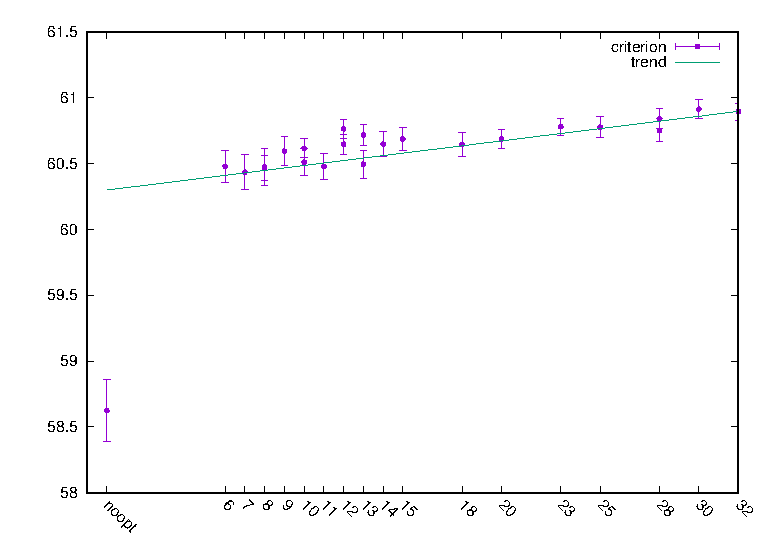
\includegraphics{mcvs025}

\caption{Evaluation of optimal policies. Points: average value of $-\rho$, bars: standard deviations, line: trend $a+b\kappa$. The horizontal axis -- labels: $k_1$ and $k_2$, positions: $k_1+k_2$. }


\label{fig:mcvs}
\end{center}
\end{figure}

\begin{figure}
\begin{center}
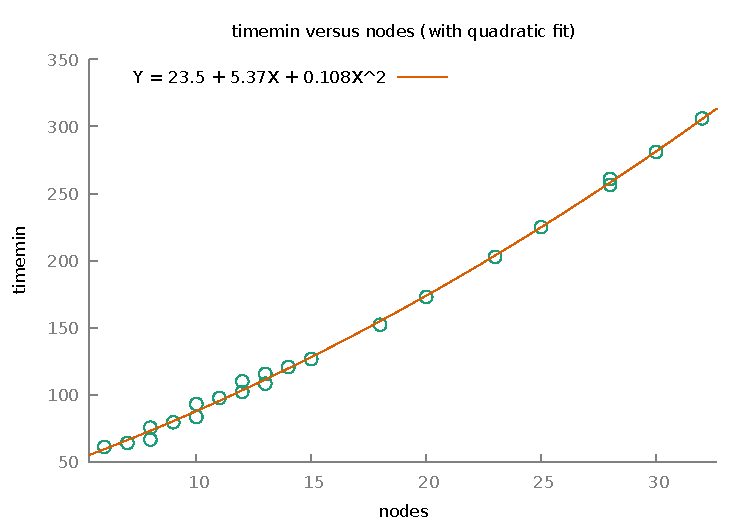
\includegraphics{times}\caption{Computational times in dependence on $\kappa$. Vertical axis: time in seconds. }
\label{fig:times}

{\tt TBD(Cherri, Antonin, please leave this mark here, we delete it later. Anyway, for consistency with Table 1, I would convert it into minutes. Moreover, always for
sake of consistency and readability, I would format the horizontal axis exactly as done for
Figure 2 and Figure 3.)}
\end{center}
\end{figure}

Clearly, once the true optimal value $v$ is finite, the trend of the criterion improvement
cannot be linear in $\kappa$ as the series should converge
to $v$ from below. Unfortunately, the noise of the estimation
prevented us from fitting more complex trends. However, when we rerun
the same analysis with all the processes except for $P$
deterministic, the noisedness of the criterion estimation decreased enough for the non-linear regression
\[
v-\tilde{v}_{k_1,k_2}\sim a\exp\{b\kappa\}
\]
to be significant, giving $v=63.46(0.06)$, $a=2.40(0.11)$, $b=-0.092(0.009)$, see also Figure \ref{fig:mcvs0}. This suggests that the convergence
rate of the approximation error as $\kappa\rightarrow \infty$ is exponential (a similar model with
$v-\tilde{v}=O(\kappa^{b})$ came out insignificant). 

\begin{figure}
\begin{center}
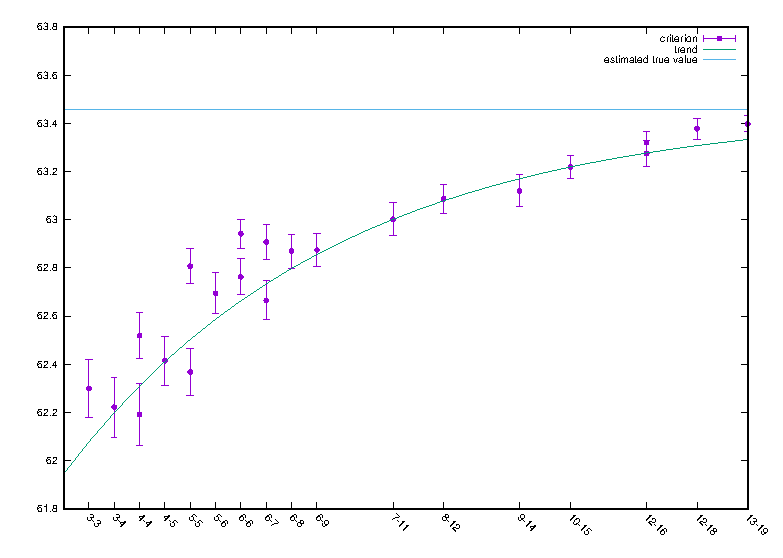
\includegraphics{mcvs0}
\caption{Evaluation of optimal policy with $\eta$ deterministic.}
\label{fig:mcvs0}
\end{center}
\end{figure}


Finally, as an experiment, we run several optimizations with discrete
approximations and tried to evaluate them the same way as the smoothed
quantization. In particular, we used the skeleton process $\varepsilon$
calibrated to be a martingale as an approximation instead of $\varsigma$.
The resulting optimal policies, however, showed to be useless because they recommended
arbitrage as a reaction to a significant portion of scenarios; needless
to say that these recommendations led mostly to huge losses ``in reality'', as the true
discounted price process is a supermartingale. This clearly speaks
in favour of the smoothed quantization. However, it should be said in
defence of discrete approximations that, when the decision period
is long, a new optimization could (and should) be done at each stage
rather then using the policy from the previous optimization; this
new optimization can clearly be calibrated not to produce arbitrage in its first stage. If, on the other hand, the decision period is
short, as in high-frequency trading for instance, then
having a policy not producing arbitrage at hand is more than necessary.

\section{Conclusions} 
\label{sec:conc}

We proposed an approximation technique suitable for multi-stage problems with Markov random parameters and we illustrated its usefulness on a realistic problem. Our technique is suitable especially for financial applications as it does not neglect the distribution tails and it can cope with arbitrage potentially arising in approximated problems. 

In the present paper, the approximation is designed to minimize nested distance; however, its  parameters may be set to meet another criteria, e.g. to keep the first two moments of the exact process (the moments of $\varsigma$ may be easily evaluated by the Law of Iterated Expectation and the Law of Iterated Variance). Inspired by \cite{kozmik2014evaluating}, one may also think of finer approximation of the tails in order to fit tail measures more accurately. 

Thinking of future research, three ideas come to our minds. First, looking at Figure \ref{fig:ilust1}, it suggests itself to set $\P[\varepsilon_{t}=\bullet|\varepsilon_{t-1}=e]$ so that $\d(\nu_{t}(e),\mu_t(e))$ is minimized rather than determine the probabilities by (\ref{eq:skelet}). It should be, however, noted that such minimization could be difficult and, moreover, some of our theoretical results would stop holding. Second, our ``anti-arbitrage protection'' could be built into the initial construction of $\varsigma$. We did not do this in the present paper as the ``anti-arbitrage'' condition is problem-dependent; however, maybe it is possible to find more general conditions precluding arbitrage and build them into the initial construction of the approximation. Third, condition 
\begin{equation}\label{eq:altaa}
P_t \geq \varrho \sigma_{t+1}(P_{t+1})
\end{equation}
 would probably suffice for boundendess of problem (\ref{eq:etp}) (as well as of similar ones); as this condition is less strict than (\ref{eq:eb}), it would lead to smaller distortions of the original approximations. However, to provin this e.g. for Problem \ref{eq:ppp} would require dealing with estimation of $\sigma_t(cM_t+dP_t)$ from below for some constants $c,d$, which would require either uniform boundedness of $M_t$, which is not the case in our example, or a general estimate of risk mappings of independent sums from below which we, however, are not aware of. But nothing prevents anyone to use approximations restricted only by (\ref{eq:altaa}) given that they do not produce arbitrage in practice.
 
Clearly, our technique may be improved many ways; however, even in the present form, it may be useful for a wide area of problems, including portfolio selection, derivative replication or asset-liability management. 


\section*{Acknowledgments}

This work was supported by Grant No. GA21-07494S of the Czech Science Foundation. The support is gratefully acknowledged.

\section*{Declarations}

\subsection*{Competing Interests}

The authors declare no competing interests.

\subsection*{Data Availability Statement}

All the data used in the paper are either published in the text or freely available.



%\bibliographystyle{informs2014}
\bibliographystyle{plainnat}
\bibliography{smid,vasek}


\appendix

\section{Auxiliarry Results}
 
 
\begin{lemma}
\label{lem:cw}Let $1<t\leq T$ and let $\xi,\varsigma$ be processes on $\{1,\dots,t\}$ taking values in $\R^p$. 
Denote $P=\L$($\barxi_{t}$), $Q=\L(\barvs_{t})$.
Let $\pi$ be a nested transportation from $P$ into $Q$. Then, for
each $x,s\in\R^{\bar{p}_{t-1}}$, an optimal transportation $\varpi_{t}(\bullet|x,s)$
from $P[\xi_{t}\in\bullet|\barxi_{t-1}=x]$ into $Q[\varsigma_{t}\in\bullet|\barvs_{t-1}=s]$
(w.r.t. $\dw$) exists and, moreover $\varpi_{t}$ is a probability
kernel.
\end{lemma}

\begin{proof}
By \cite{villani2003topics}, Theorem 1.3. $\varpi_{t}(\bullet|x,s)$
exists (and is a probability measure) for each $x,s$. To prove that
$\varpi_{t}$ is a probability kernel, it remains to show that
\begin{equation}
\text{\ensuremath{\varpi_{t}(A|\bullet)} is measurable for each \ensuremath{A\in\B^{p}\otimes\B^{p}.}}\label{eq:vpm}
\end{equation}
Certainly, (\ref{eq:vpm}) holds if $A\in\C,$ $\C=\{B\times C:B,C\in\B^{p},\text{ at least one of $B$ and $C$ is $\R^p$}\}$
(because $\varpi_{t}(A|\bullet)=\P[B|\xi_{t-1}=\bullet_{1}]$ which
is measurable by definition, similarly for the second coordinate).
Clearly, $\C$ is a $\pi$ system with $\sigma(\C)=\B^{p}\otimes\B^{p}$.
Put $\mathcal{D=}\{A\in\B^{p}\otimes\B^{p}:A\text{ fulfils (\ref{eq:vpm})}\}.$
Trivially, $\R^{p}\times\R^{p}\in\mathcal{D}$. Further, once
$A,B\in\mathcal{D}$ and $B\subset A$, we have $\varpi_{t}(A\setminus B|\bullet)=\varpi_{t}(A|\bullet)-\varpi_{t}(B|\bullet)$
(by the elementary properties of probability measures), so $A\setminus B\in\mathcal{D}$
by \cite{Kallenberg02}, Lemma 1.12. Finally, once 
for $A_{1}\subset A_{2}\subset\dots$, $A_{i}\in\mathcal{D}$, $i\in \N$, we have $\lim_{i}A_{i}\in\mathcal{D}$
by \cite{Kallenberg02}, Lemmas 1.14 and 1.10 (ii). Thus, $\mathcal{D}$
is a $\lambda$-system containing $\C$, and, by the Monotone Class
Argument (\cite{Kallenberg02}, Theorem 1.1), $\B^{p}\times\B^{p}\in\mathcal{D}$,
i.e. (\ref{eq:vpm}) holds true.
\end{proof}
 
 
\begin{lemma}
\label{lem:flemma}Let $\mu$ be a conditional distribution on $(\R^{p},\B^{p})$ given values from from a measurable
space $(S,\mathcal{S})$. Let $U\in\R^{s}$
be a random vector and let $g:S\times R^{s}\rightarrow\R^{p}$ be
a measurable mapping such that 
\begin{equation}
\mu(\bullet|x)=\P[g(x,U)\in\bullet].\label{eq:gut}
\end{equation}
Then
\[
\mathrm{d}(\mu(x),\mu(y))\leq\int\|g(x,u)-g(y,u)\|\L(U)(du).
\]
\end{lemma}

\begin{proof}
Fix $x,y\in S$. Put
\[
X=\zeta(U),\qquad 
\zeta:(\R^{s},\B^{s})\rightarrow(S\times S,\mathcal{S}\otimes\mathcal{S}),\qquad\zeta(u)=(g(x,u),g(y,u)),
\]
and denote $\pi=\L(X)$. As
\[
\pi(\bullet\times S)=\P[\zeta(U)\in\bullet\times S]=\P[g(x,U)\in\bullet]=\mu(\bullet|x)
\]
and, similarly, $\pi(S\times\bullet)=\mu(\bullet|y)$, $\pi$ is a
transportation from $\mu(x)$ to $\mu(y)$. Moreover, by calculus,
\[
\int\|r-s\|\pi(dr,ds)=\int\|g(x,u)-g(y,u)\|\L(U)(du)
\]
which proves the Lemma because the l.h.s. majorizes the Wasserstein
distance. 
\end{proof}

\begin{lemma}
\label{lem:ddd}For any processes $\xi,\varsigma$ in $\R^{p}$ and
any $1\leq t,$
\[
\dw(\xi_{t},\varsigma_{t})\leq\dw(\barxi_{t},\barvs_{t})\leq\d(\barxi_{t},\barvs_{t})
\]
\end{lemma}

\begin{proof}
Let $\pi$ be the optimal transportation from $\barxi_{t}$ to $\barvs_{t}$.
Then $\pi_{t}(X,S)\defined \pi(\R^{(t-1)p}\times X,\R^{(t-1)p}\times S)$
is a transportation from $\xi_{t}$ to $\varsigma_{t}$ which proves the
first inequality. For the second one, see \cite{pflug2014multistage},
Lemma 2.37.
\end{proof}
 
\begin{lemma}
\label{lem:indep}Let  $q\in \N$ and let $\eta,\eta'$ be processes on ${0,\dots,T}$ with $\eta_{t},\eta'_{t}\in$$\R^{q}$, $0\leq t\leq T$, 
having the same distribution, 
with $\eta_{0}=\eta'_{0}$
deterministic, such that $\eta\indep{\xi}$, \textup{$\eta'\indep{\varsigma}$.
}Then $\d((\xi,\eta),(\varsigma,\eta'))\leq\d(\xi,\varsigma)$.
\end{lemma}

\begin{proof}
Let $\rho$ be a nested transportation, $\epsilon$-optimal with respect
to $\d(\xi,\varsigma)$. For any $1\leq t\leq T$, denote $\rho_t$ the transportation from $\xi_t|\barxi_{t-1}$ to 
$\varsigma_t|\barvs_{t-1}$ (its existence is assured by the definition of the nested transportation).

Further, for each $t$ and $\baru,\overline{v}\in\R^{\bar{q}_{t-1}},$$\bar{q}_{t-1}=(t-1)q$,
let $\sigma_{t}(\bullet|\baru,\overline{v})$ the optimal transportation
from $\L(\eta_{t}|\overline{\eta}_{t-1}=\baru)$ into $\L(\eta_{t}|\overline{\eta}_{t-1}=\overline{v})$.
By Lemma \ref{lem:cw}, $\sigma_{t}$ is well defined probability
kernel. As $\dw$ is a metric, we have $0=\dw(\eta_{t}|\baru,\eta'_{t}|\baru)=\int\|u-v\|\sigma{}_{t}(du,dv|\baru,\baru)$, so we can choose $\sigma_{t}$ so that $\sigma_{t}(\bullet|\baru,\baru)$
is concentrated on $\{(u,u):u\in\R^{q}\}$.

For any $1\leq t\leq T$, denote $\theta=(\xi,\eta),$$\theta'=(\varsigma,\eta')$
and consider a conditional distribution $\pi_t$ fulfilling
\[
\pi_{t}(\xi_{t}\in A,\eta_{t}\in B,\varsigma_{t}\in C,\eta'_{t}\in D|\overline{\theta}_{t-1},\overline{\theta'}_{t-1})=\sigma_{t}(B\times D|\overline{\eta}_{t-1},\overline{\eta'}_{t-1})\otimes\rho_{t}(A\times C|\barxi_{t-1},\barvs_{t-1}).
\]
It could be easily proved by the Monotone Class Argument (see the
proof of Remark \ref{rem:cpp}) in Appendix that $\pi_{t}$ is a transportation
from $\theta_{t}|\overline{\theta}_{t-1}$ into $\theta'_{t}|\overline{\theta'}_{t-1}$.
Consequently, the distribution $\pi$ defined by the composition of
$\pi_{1},\dots,\pi_{T}$ is a nested transportation, so we have
\begin{multline*}
\d(\theta,\theta')\leq\int\|\bary_{T}-\overline{z}_{T}\|\pi(d\bary_{T},d\overline{z}_{T})\\
=\int\dots\int(\|\barx_{T}-\bars_{T}\|+\|\baru_{T}-\overline{v}_{T}\|)\sigma_{T}(du_{T},dv_{T}|\baru_{T-1},\overline{v}_{T-1})\rho_{T}(dx_{T},ds_{T}|\barx_{T-1},\bars_{T-1})\dots\\
\sigma_{1}(u_{1},v_{1})\rho_{t}(x_{1},s_{1})\\
=\int\|\baru_{T}-\overline{v}_{T}\|\sigma_{T}(du_{T},dv_{T}|\baru_{T-1},\overline{v}_{T-1})\dots\sigma_{1}(u_{1},v_{1})
\\
\qquad\qquad +\int\|\barx_{T}-\bars_{T}\|\rho_{T}(dx_{T},ds_{T}|\barx_{T-1},\bars_{T-1})\dots\rho_{t}(x_{1},s_{1})\\
=0+\int\|\barx_{T}-\bars_{T}\|\rho_{T}(d\barx_{T},d\bars_{T})\leq\d(\xi,\varsigma)+\epsilon.
\end{multline*}
The Lemma now follows by limit transition.
\end{proof}
 

\section{Proofs}

\subsection{Proof of Remark \ref{rem:cpp}}

\label{app:cpp}

By the Tower Property (\cite{pflug2012distance}, Lemma 10), $\pi$
is a nested transportation in the sense of \cite{pflug2012distance}
if and only if, for each $1\leq t\leq T$,
\begin{equation}
\pi((\barxi_{t},\barvs_{t})\in A\times\R^{\bar{p}_{t}}|\barxi_{t-1},\barvs_{t-1})=P[\barxi_{t}\in A|\barxi_{t-1}],\qquad A\in\B^{\bar{p}_{t}},\label{eq:ppp}
\end{equation}
\begin{equation}
\pi((\barxi_{t},\barvs_{t})\in\R^{\bar{p}_{t}}\times B|\barxi_{t-1},\barvs_{t-1})=Q[\barvs_{t}\in B|\barvs_{t-1}],\qquad B\in\B^{\bar{p}_{t}}.\label{eq:qpp}
\end{equation}
Applying (\ref{eq:ppp}) to sets $A=A_{t}\times\R^{\overline{p}_{t-1}}$,
$A_{t}\in\B^{p}$, 
%and $B=B_{t}\times\R^{\overline{p}_{t-1}}$, $B_{t}\in\B^{p}$,
we see that (\ref{eq:ppp}) implies (\ref{eq:tpp}). To prove the
reverse implication, note first that (\ref{eq:tpp}) implies (\ref{eq:ppp})
for any $A\in\C\defined\{B\times C:B\in\B^{p}$, $C\in\B^{\bar{p}_{t-1}}\}$;
indeed, 
\begin{multline*}
P[\barxi_{t}\in A|\barxi_{t-1}]=\E_{P}(\charf_{B}(\xi_{t})\charf_{C}(\barxi_{t-1})|\barxi_{t-1})\\
=\charf_{C}(\barxi_{t-1})P[\xi_{t}\in B|\barxi_{t-1}]=\charf_{C}(\barxi_{t-1})\pi[(\xi_{t},\varsigma_{t})\in B\times\R^{p}|\barxi_{t-1},\barvs_{t-1}]\\
=\charf_{C}(\barxi_{t-1})\E_{\pi}(\charf_{B}(\xi_{t})|\barxi_{t-1},\barvs_{t-1})=\E_{\pi}(\charf_{C}(\barxi_{t-1})\charf_{B}(\xi_{t})|\barxi_{t-1},\barvs_{t-1})\\
=\pi[(\barxi_{t},\barvs_{t})\in A\times\R^{\bar{p}_{t}}|\barxi_{t},\barvs_{t}]
\end{multline*}
(we used the pull-out property of conditional expectations (\cite{Kallenberg02}, Theorem 6.1 (v)) twice).
As, by the definition of the product sigma fields, $\C$ is a generator
of $\B^{\bar{p}_{t}}$, closed under finite intersections, and as
the system of sets $A$ fulfilling (\ref{eq:ppp}) contains $\R^{\bar{p}_{t}}$
and is closed under proper differences and increasing limits (by the
properties of probability measures\footnote{Here, the proof would fail if the conditional probabilities were not
regular because the conditional probabilities which are not regular
need not be probability measures.}), (\ref{eq:tpp}) follows by the Monotone Class Argument (\cite{Kallenberg02},
Theorem 1.1.). The proof of the equivalence of (\ref{eq:qpp}) and
(\ref{eq:tpq}) is symmetric. 

\subsection{Proof of Proposition \ref{prop:pp}}

\label{app:pp}

Let $\pi_{t-1}$ be an $\epsilon$-optimal (w.r.t. $\d(\barxi_{t-1},\barvs_{t-1})$)
nested transportation from $\barxi_{t-1}$ to $\barvs_{t-1}$. Let,
for each $x,s\in\R^{p}$, $\varpi_{t}(\bullet|x,s)$ be the optimal
transportation from $\mu(x)$ into $\nu(s)$; by Lemma \ref{lem:cw} (Appendix),
$\varpi_{t}$ is a well defined probability distribution.

Put
\[
\pi_{t}(d\barx_{t},d\bars_{t})=\varpi_{t}(dx_{t},ds_{t}|x_{t-1},s_{t-1})\pi_{t-1}(d\barx_{t-1},d\bars_{t-1}).
\]
As, by the Markov property, $\mu_{t}(\xi_{t-1})=\L(\xi_{t}|\barxi_{t-1})$,
$\nu_{t}(\varsigma_{t-1})=\L(\varsigma_{t}|\overline{\varsigma}_{t-1})$,
and as, by definition, $\varpi_{t}$ is a conditional distribution
of the last $2p$ components of $\pi_{t}$, we have, by Definition
\ref{dt}, that $\pi_{t}$ is a nested transportation from $\barxi_{t}$
to $\barvs_{t}$. Thus 
\begin{multline}
\d(\barxi_{t},\barvs_{t})\leq\int\|\barx_{t}-\bars_{t}\|\pi_{t}(d\barx_{t},d\bars_{t})\\
=\int\int[\|\barx_{t-1}-\bars_{t-1}\|+\|x_{t}-s_{t}\|]\varpi_{t}(dx_{t},ds_{t}|x_{t-1},s_{t-1})\pi_{t-1}(d\barx_{t-1},d\bars_{t-1})\\
\leq\d(\barxi_{t-1},\barvs_{t-1})+\epsilon+B_{t},\label{eq:dxs}
\end{multline}
where
\begin{multline*}
B_{t}=\int\left(\int\|x{}_{t}-s_{t}\|\varpi_{t}(dx_{t},ds_{t}|x_{t-1},s_{t-1})\right)\pi_{t-1}(d\barx_{t-1},d\bars_{t-1})\\
=\mathrm{\int d}(\mu_{t}(x_{t-1}),\nu_{t}(s_{t-1}))\pi_{t-1}(d\barx_{t-1},d\bars_{t-1})\\
\leq\int\mathrm{d}(\mu_{t}(x_{t-1}),\mu_{t}(s_{t-1}))\pi_{t-1}(d\barx_{t-1},d\bars_{t-1})\\
\qquad\qquad+\int\mathrm{d}(\mu(s_{t-1}),\nu_{t}(s_{t-1}))\pi_{t-1}(d\barx_{t-1},d\bars_{t-1})\\
\leq K_{t}\int\|x_{t-1}-s_{t-1}\|\pi_{t-1}(d\barx_{t-1},d\bars_{t-1})+\E d(\mu_{\tau}(\varsigma_{\text{\ensuremath{\tau}}-1}),\nu_{\tau}(\boldsymbol{\varsigma}_{\tau-1}))\\
\leq K_{t}(\mathrm{\d}(\barxi_{t-1},\barvs_{t-1})+\epsilon)+\E d(\mu_{\tau}(\varsigma_{\text{\ensuremath{\tau}}-1}),\nu_{\tau}(\boldsymbol{\varsigma}_{\tau-1}))
\end{multline*}
(we have used the triangular inequality for $\dw$). The Proposition
now follows by imposing this into (\ref{eq:dxs}) and by a limit transition. 


\end{document}
 





%%%%%%%%%%%%%%%%%%%%%%%%%%%%%%%%%%%%%%%%%%%%%%%%%%%%%%%%%%%%%%%%%%%%%%

% Samples of sectioning (and labeling) in MOOR.
% NOTE: (1) all section levels end with a period,
%       (2) capitalization is as shown (sentence style, not title style).
%
%\section{Introduction.}\label{intro} %%1.
%\subsection{Duality and the classical EOQ problem.}\label{class-EOQ} %% 1.1.
%\subsection{Outline.}\label{outline1} %% 1.2.
%\subsubsection{Cyclic schedules for the general deterministic SMDP.}
%  \label{cyclic-schedules} %% 1.2.1
%\section{Problem description.}\label{problemdescription} %% 2.

% Text of your paper here

% Appendix here
% Options are (1) APPENDIX (with or without general title) or 
%             (2) APPENDICES (if it has more than one unrelated sections)
% Outcomment the appropriate case if necessary
%
%
%   or 
%
% \begin{APPENDICES}
% \section{<Title of Section A>}
% \section{<Title of Section B>}
% etc
% \end{APPENDICES}


% Acknowledgments here
% Enter the text of acknowledgments here

% References here (outcomment the appropriate case) 

% CASE 1: BiBTeX used to constantly update the references 
%   (while the paper is being written).
%\bibliographystyle{informs2014} % outcomment this and next line in Case 1
%\bibliography{<your bib file(s)>} % if more than one, comma separated

% CASE 2: BiBTeX used to generate mypaper.bbl (to be further fine tuned)
%\input{mypaper.bbl} % outcomment this line in Case 2

\end{document}


